\section{Hiện thực}
\label{chap:Implementation}

\subsection{Đăng nhập - Đăng ký}
$\indent$Trang đăng nhập được thiết kế để người dùng có thể đăng nhập vào tài khoản của họ. Giao diện bao gồm một form đăng nhập với hai trường nhập liệu cho tên người dùng và mật khẩu, cùng với nút "Đăng nhập". Trang cũng cung cấp liên kết "Quên mật khẩu" để người dùng khôi phục mật khẩu nếu cần, và liên kết "Đăng ký" để chuyển hướng người dùng đến trang đăng ký.
    \begin{figure}[H]
        \begin{center}
        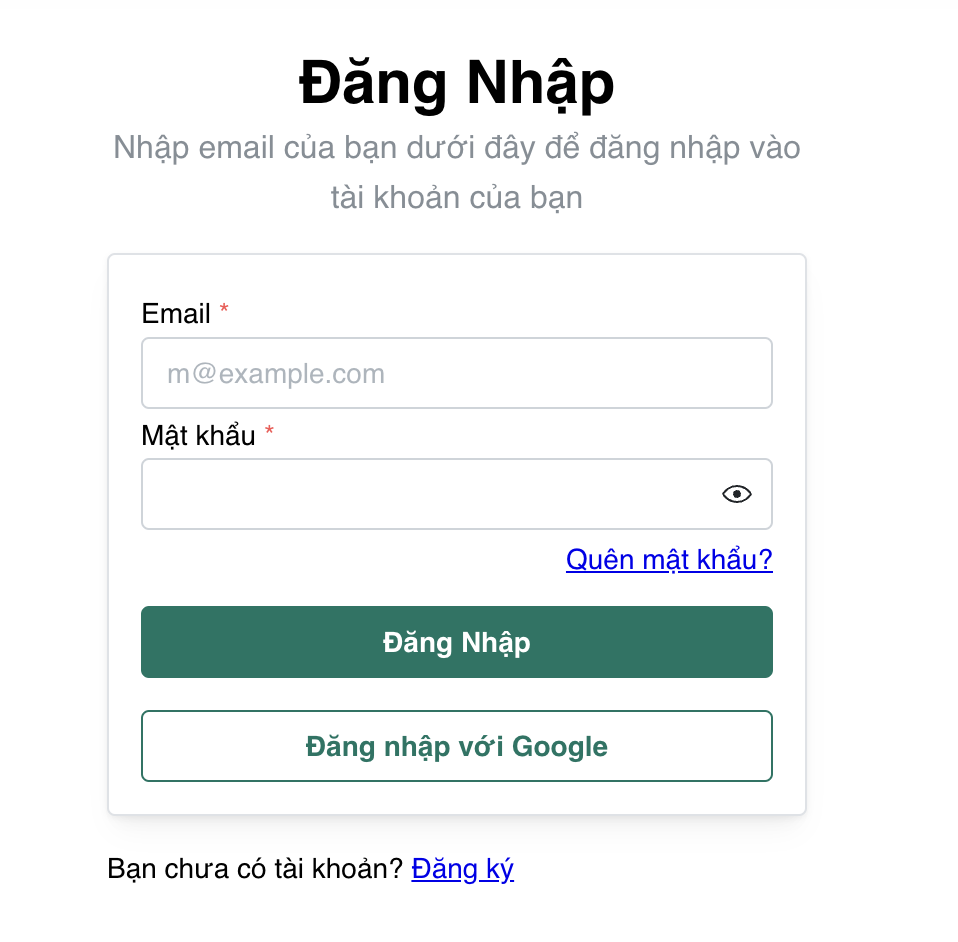
\includegraphics[width=0.6\linewidth]{Images/UI/signin.png}
        \end{center}
        \caption{Trang đăng nhập}
    \end{figure}
Trang đăng ký cho phép người dùng tạo một tài khoản mới trên hệ thống. Trang có cấu trúc tương tự với trang đăng nhập, bao gồm form đăng ký với các trường nhập liệu cho tên người dùng, địa chỉ email, mật khẩu và xác nhận mật khẩu, cùng với nút "Đăng ký". Ngoài ra, trang cũng cung cấp liên kết "Đăng nhập" để người dùng có thể chuyển hướng đến trang đăng nhập.
\begin{figure}[h]
    \centering
    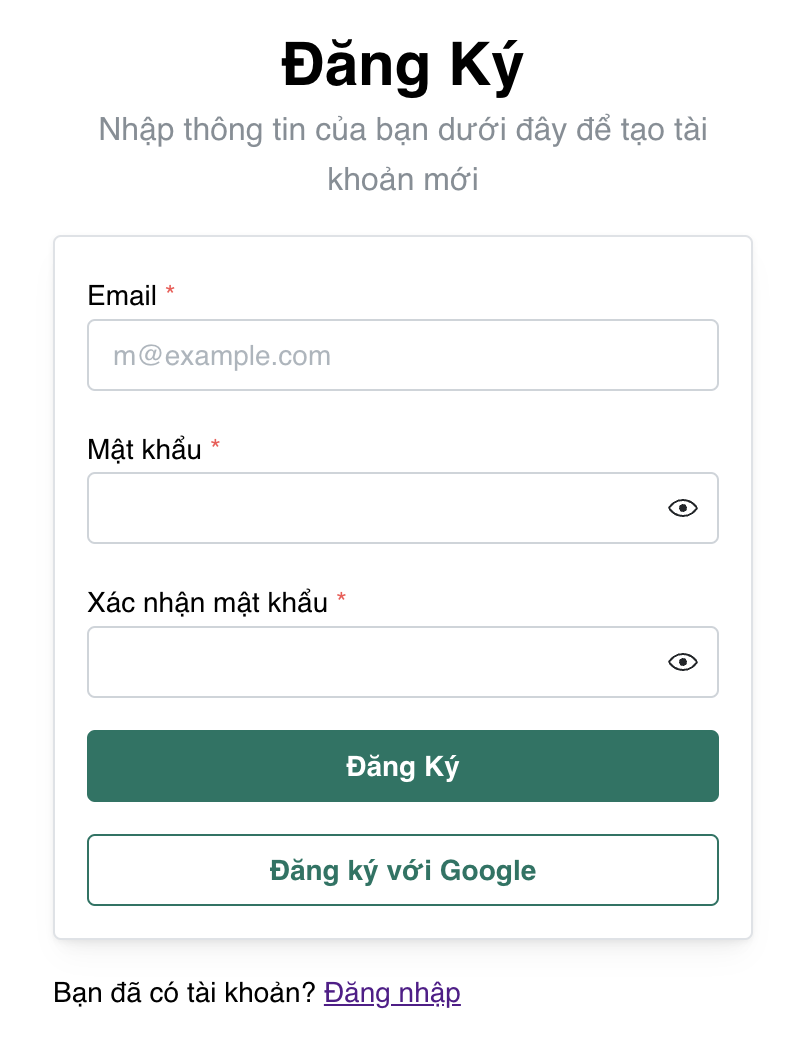
\includegraphics[width=0.5\linewidth]{Images/UI/signup.png}
    \vspace{1em}
    \caption{Trang đăng ký}
\end{figure}

\newpage
\subsection{Trang chủ}
$\indent$Trang chủ hiển thị thông tin tổng quan về các loại danh mục sản phẩm và danh sách các sản phẩm nông sản.     
\begin{figure}[H]
    \centering
    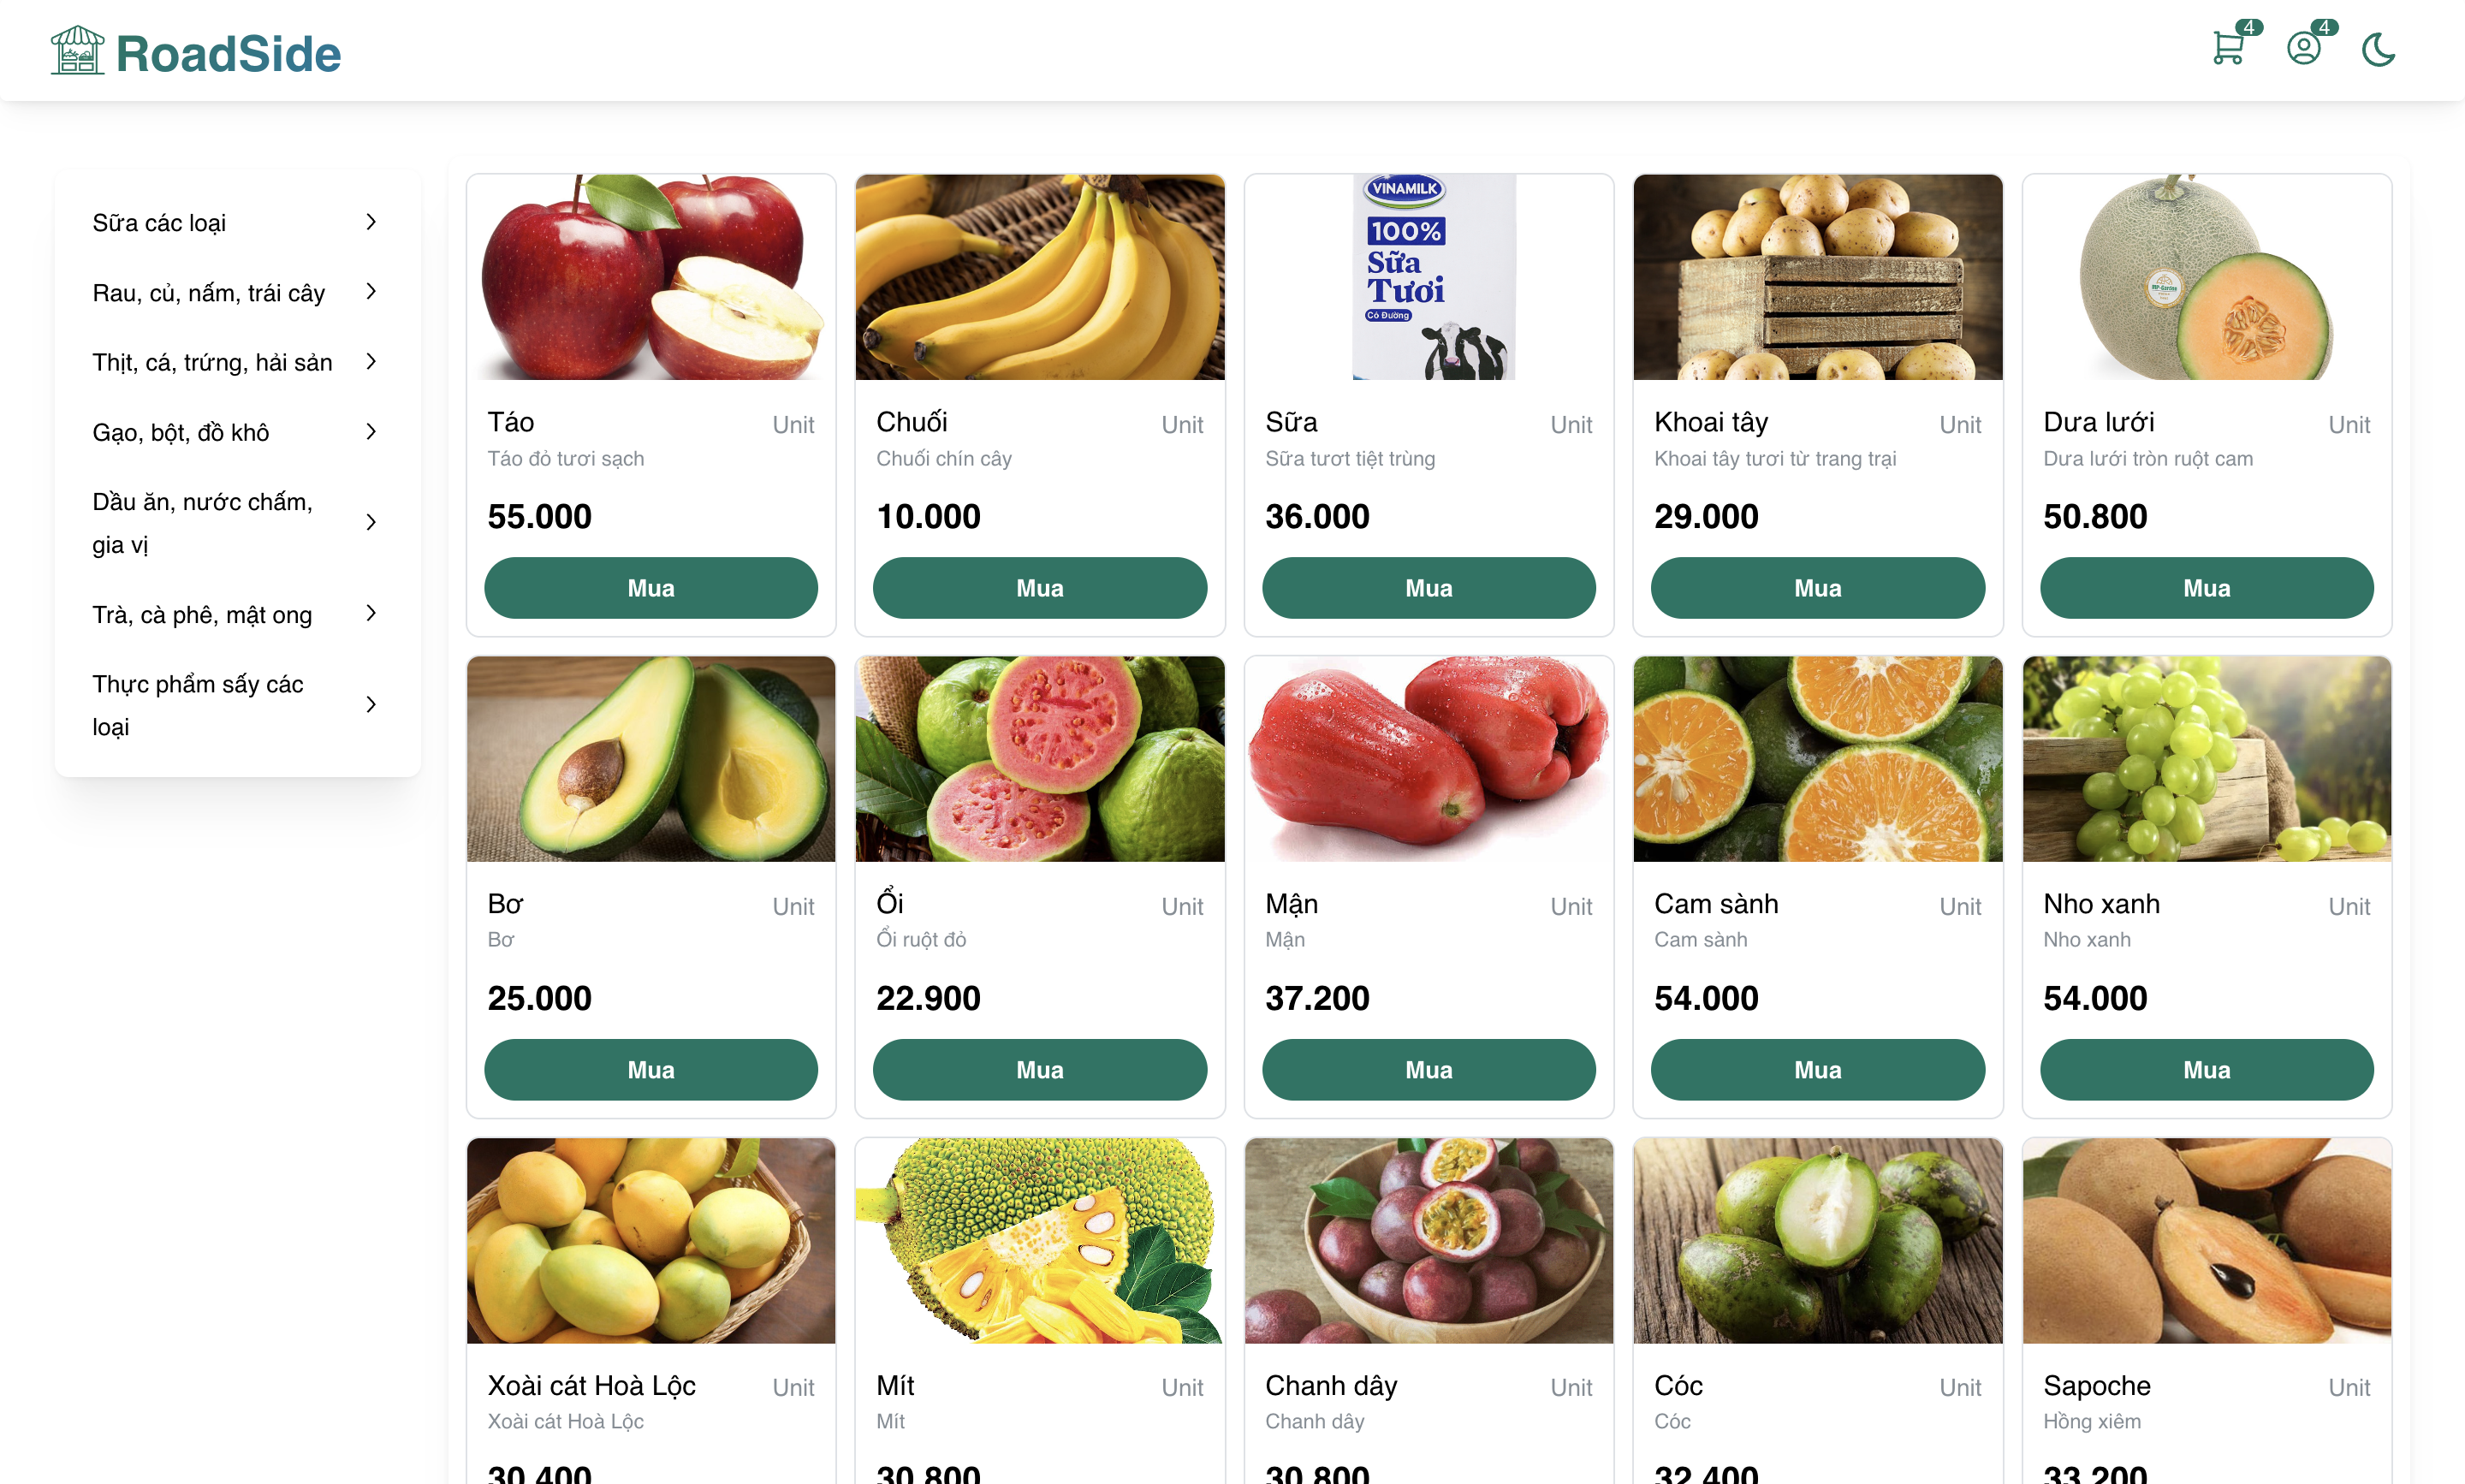
\includegraphics[scale=0.3] {Images/UI/Homepage.png}
    \vspace{2em}
    \caption{Trang chủ}
\end{figure}


Phía bên trái là danh mục các loại sản phẩm được phân loại theo từng đặc trưng riêng.
\begin{figure}[H]
    \centering
    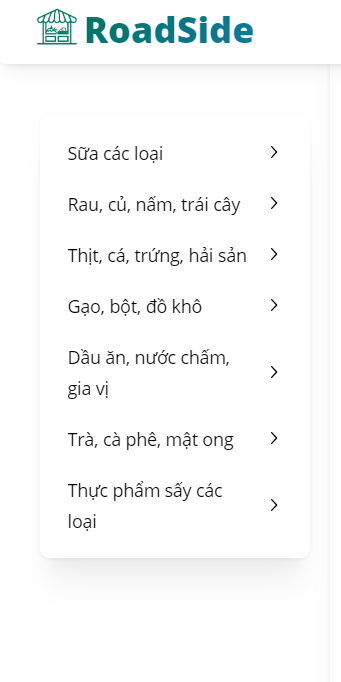
\includegraphics[scale=0.7] {Images/UI/category1.png}
    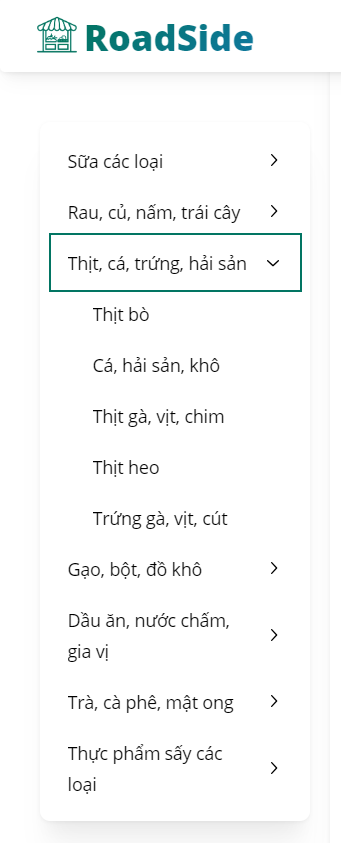
\includegraphics[scale=0.7] {Images/UI/category2.png}
    \vspace{1em}
    \caption{Danh mục sản phẩm}
\end{figure}

Sau khi chọn loại sản phẩm cần mua, danh sách các sản phẩm đã được phân loại sẽ hiện ra ở bên phải.
\begin{figure}[H]
    \centering
    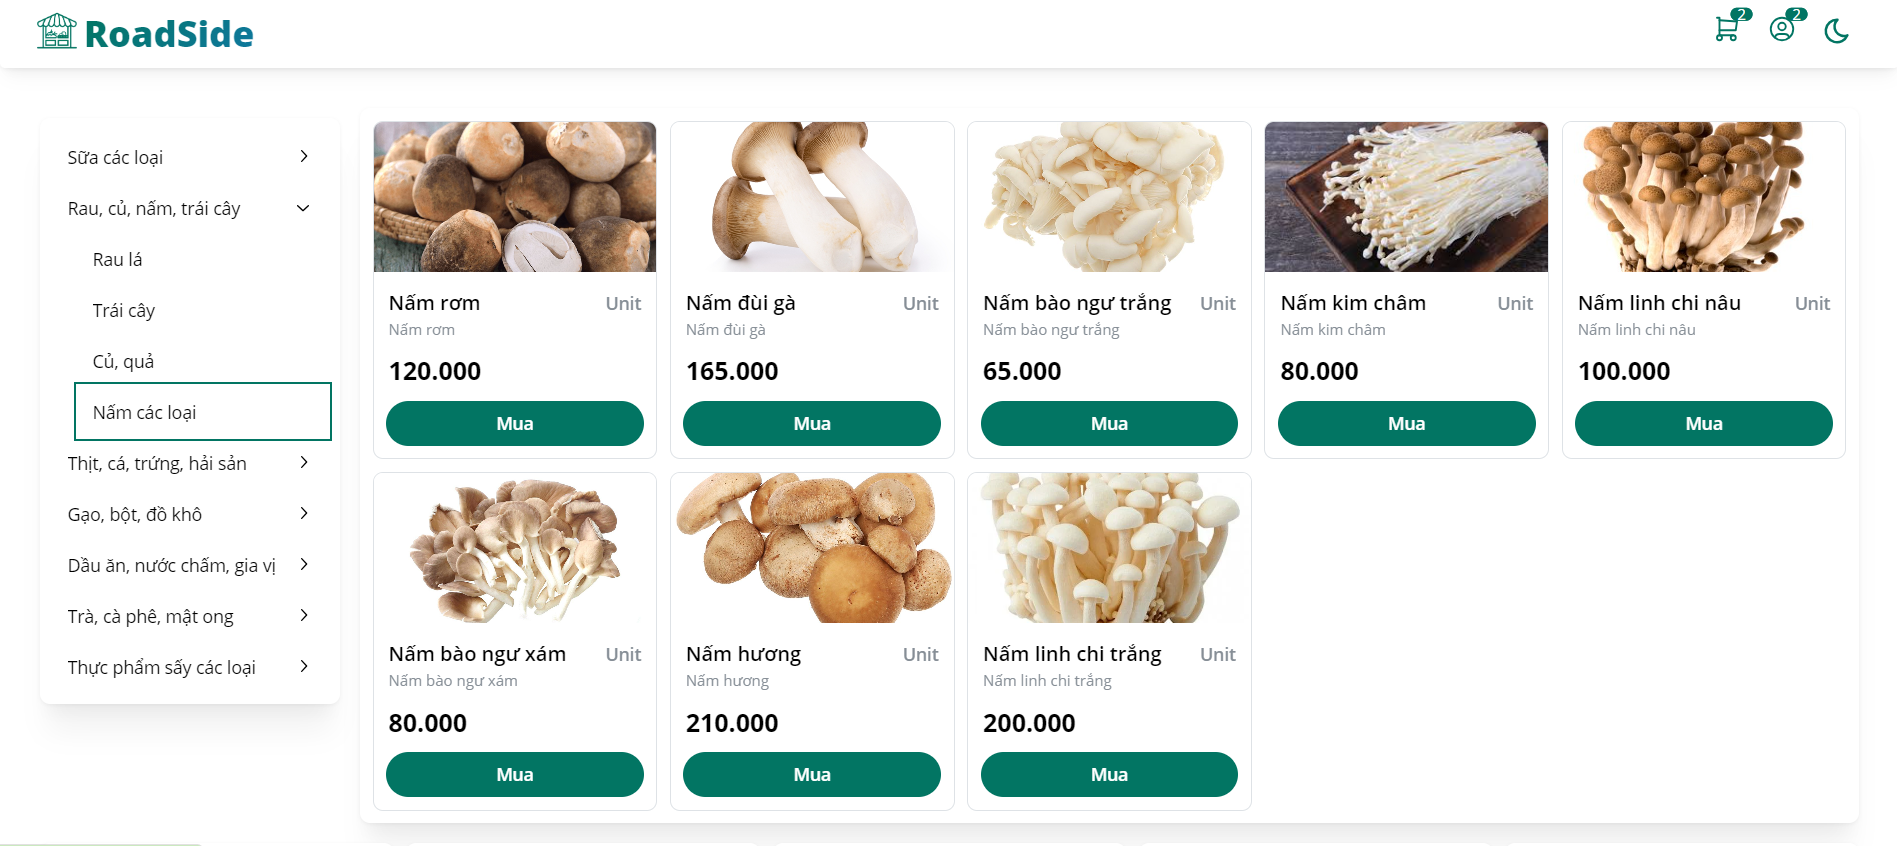
\includegraphics[width=1\linewidth] {Images/UI/product_category.png}
    \vspace{1em}
    \caption{Phân loại sản phẩm theo danh mục}
\end{figure}

\subsection{Thông tin sản phẩm}
$\indent$Ở trang chủ mỗi sản phẩm sẽ được hiển thị dưới dạng một thẻ sản phẩm, bao gồm các thông tin cơ bản như tên, giá, hình ảnh mô tả và giá giảm (nếu có).
\begin{figure}[H]
    \centering
    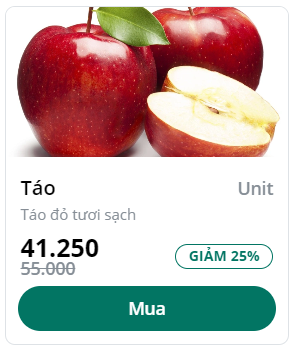
\includegraphics[scale=1] {Images/UI/product_card.png}
    \vspace{1em}
    \caption{Thẻ sản phẩm}
\end{figure}

Nếu bấm vào thẻ sản phẩm, sẽ được chuyển hướng đến trang xem thông tin chi tiết của sản phẩm đó.
\begin{figure}[H]
    \centering
    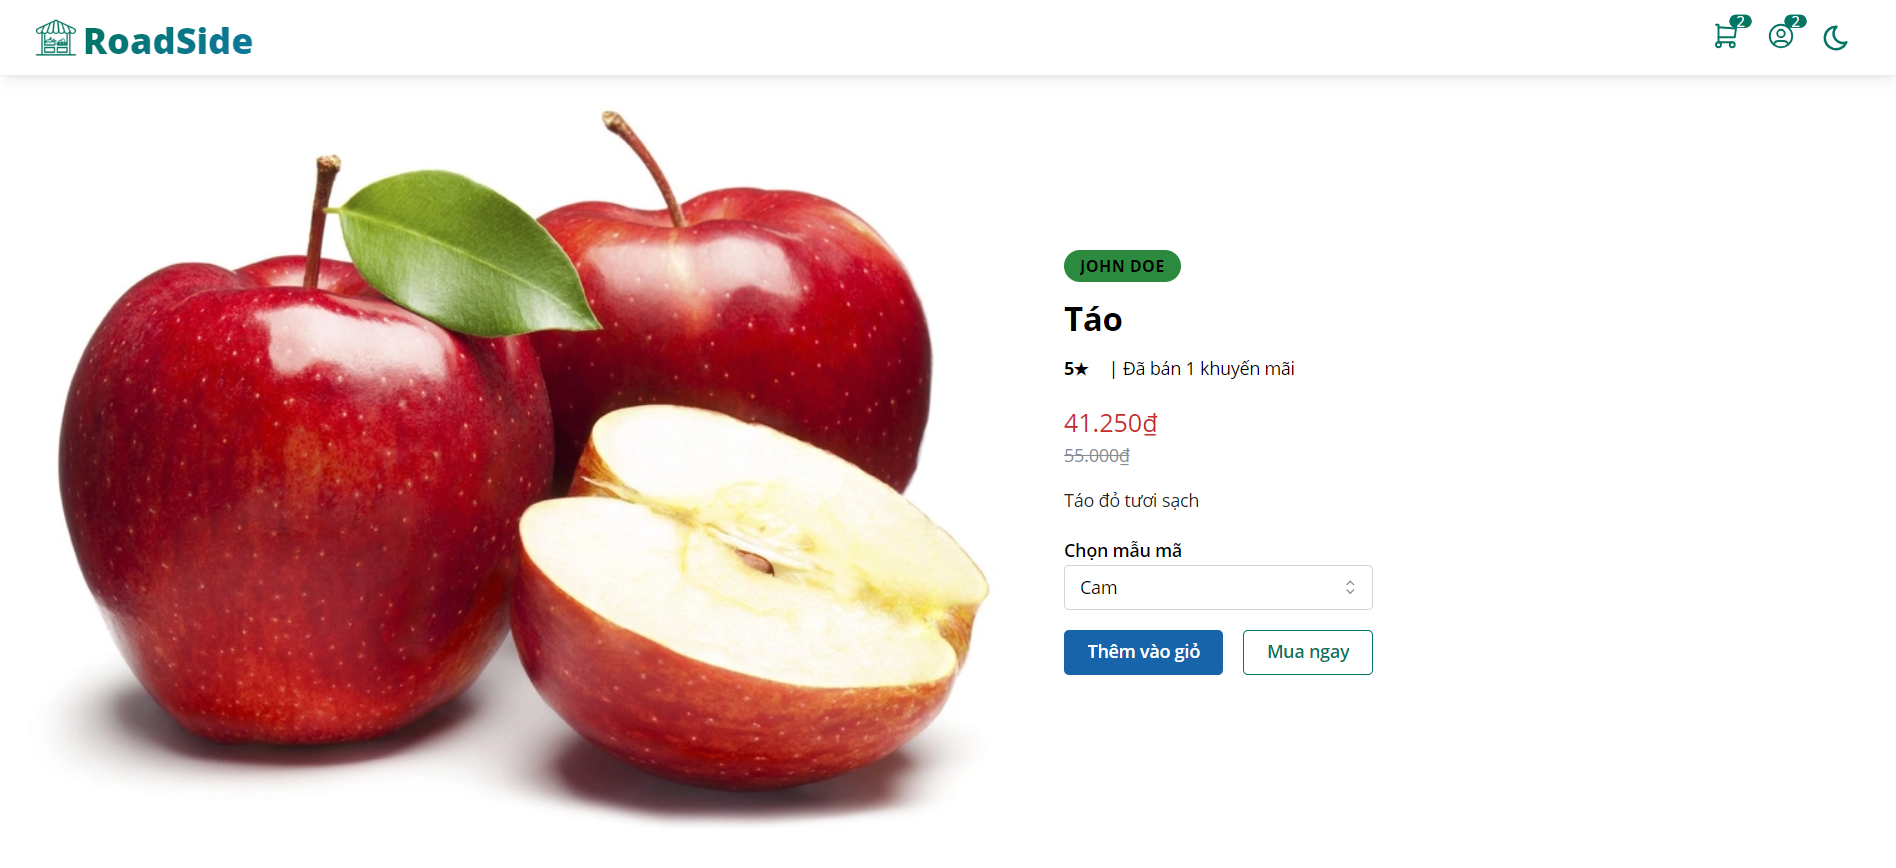
\includegraphics[width=1\linewidth] {Images/UI/product_details.png}
    \vspace{1em}
    \caption{Trang thông tin sản phẩm chi tiết}
\end{figure}

\subsection{Đặt hàng}
Sau khi đăng nhập vào hệ thống, nếu nhấn vào biểu tượng giỏ hàng trên thanh navbar, trang giỏ hàng sẽ hiện ra. Khách hàng có thể xem thông tin về các sản phẩm mà người dùng đã thêm vào giỏ hàng, bao gồm thông tin về tên, hình ảnh, giá và số lượng. Ở đây người dùng có thể xem lại và điều chỉnh các mục trong giỏ hàng trước khi đặt hàng. Người dùng có thể thay đổi số lượng hoặc xóa sản phẩm khỏi giỏ hàng.
    \begin{figure}[H]
        \centering
        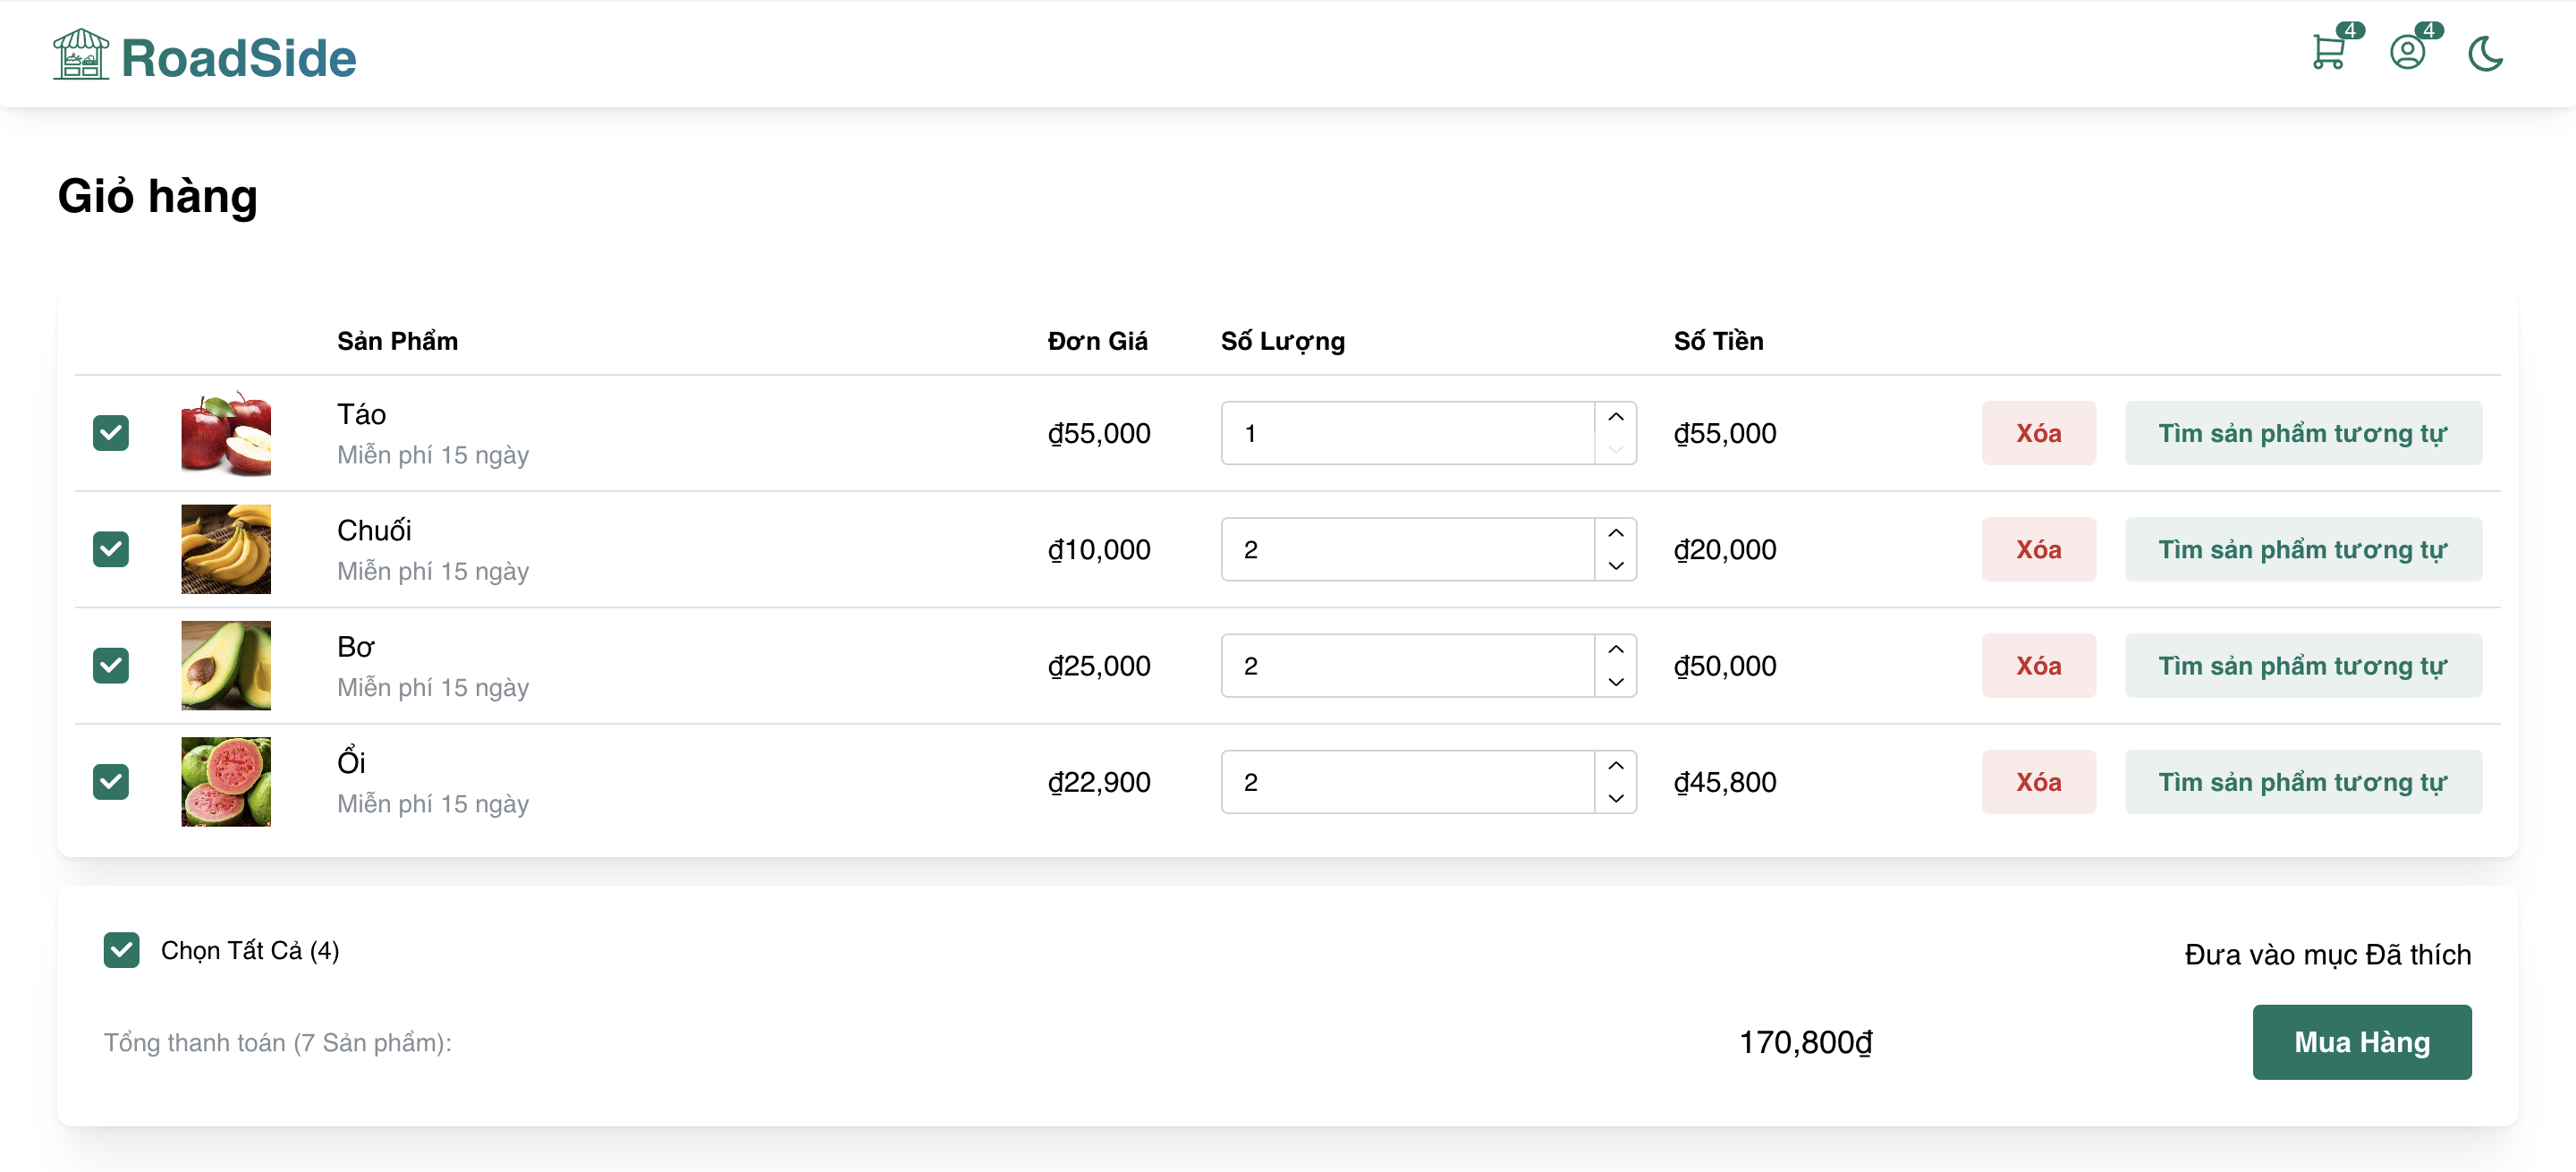
\includegraphics[width=1\linewidth] {Images/UI/cart.png}
        \vspace{1em}
        \caption{Giỏ hàng}
    \end{figure}

Bấm nút "Đặt hàng" để tiến hành tạo đơn hàng, một modal được hiện lên để xác nhận lại thông tin đặt hàng và phương thức thanh toán.

    \begin{figure}[H]
        \begin{center}
        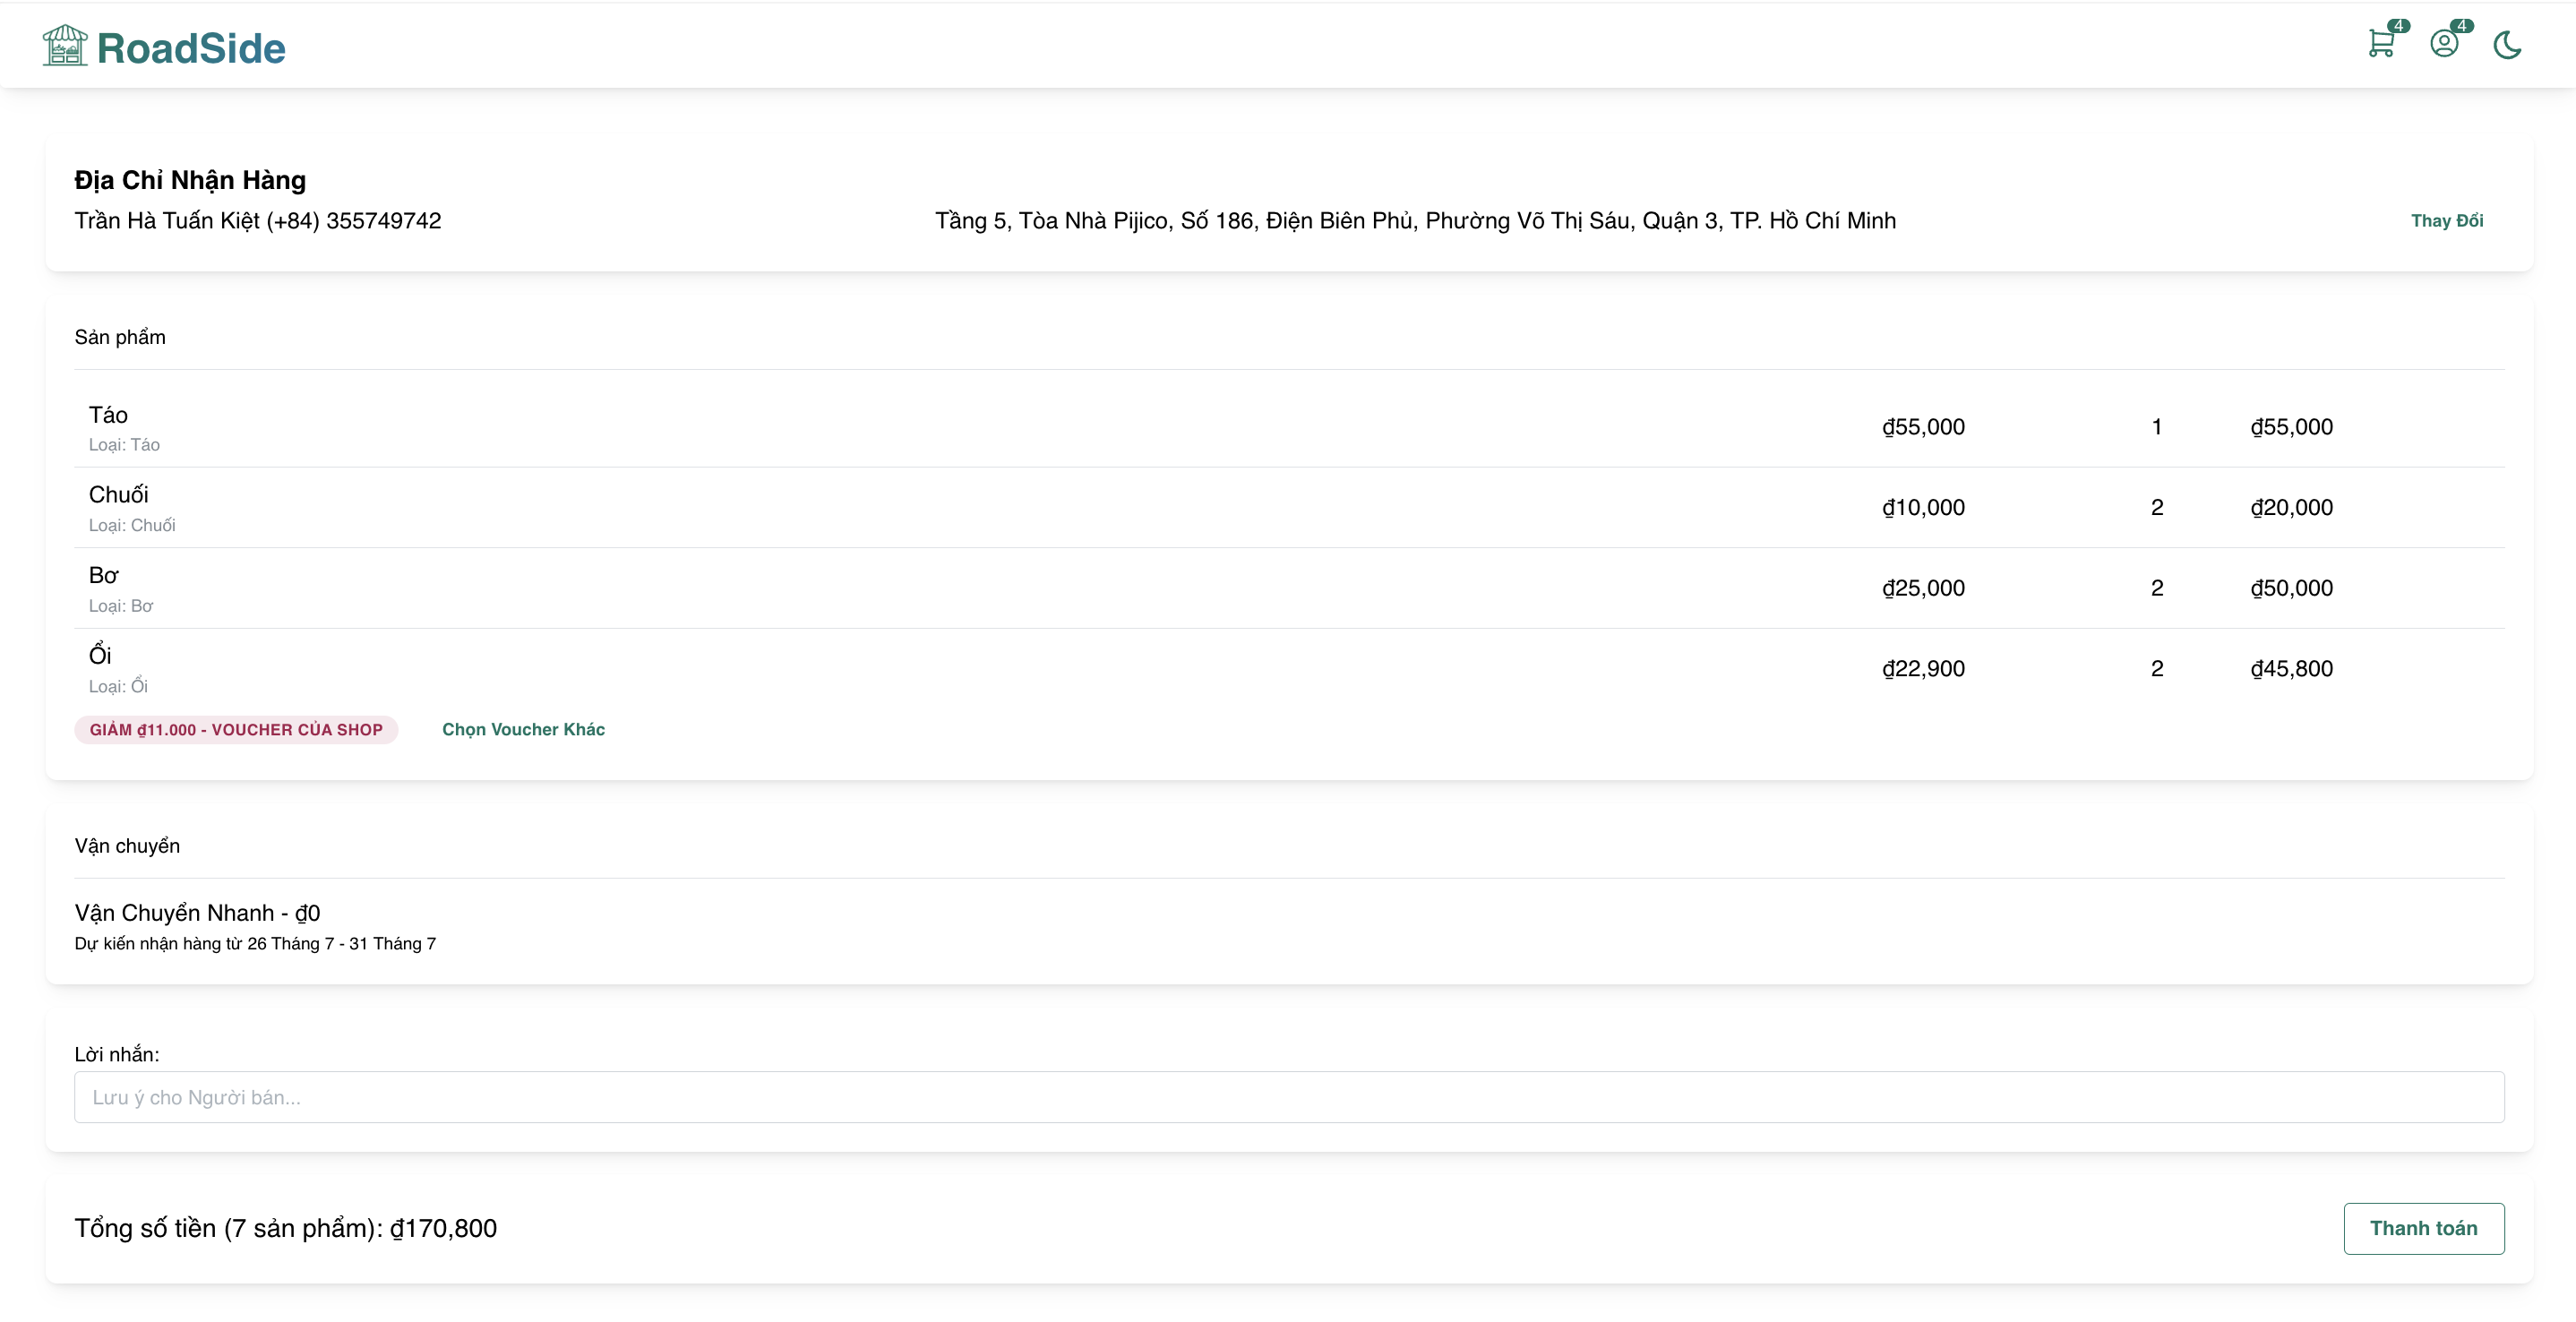
\includegraphics[scale=0.3] {Images/UI/orderform.png}
        \end{center}
        \caption{Form xác nhận đơn hàng}
    \end{figure}
Sau khi tiến hành đặt hàng và thanh toán thành công sẽ hiện thông báo đặt hàng thành công.
\subsection{Chỉnh sửa thông tin cá nhân}
Sau khi đăng nhập, người dùng có thể nhấn vào biểu tượng hình người trên thanh navbar để truy cập trang thông tin người dùng. Đây là nơi mà người dùng có thể quản lý và cập nhật thông tin cá nhân của họ. Trang này cung cấp cho người dùng một giao diện để xem và chỉnh sửa thông tin cá nhân, giúp tạo ra trải nghiệm cá nhân hóa cho khách hàng.

    \begin{figure}[H]
        \centering
        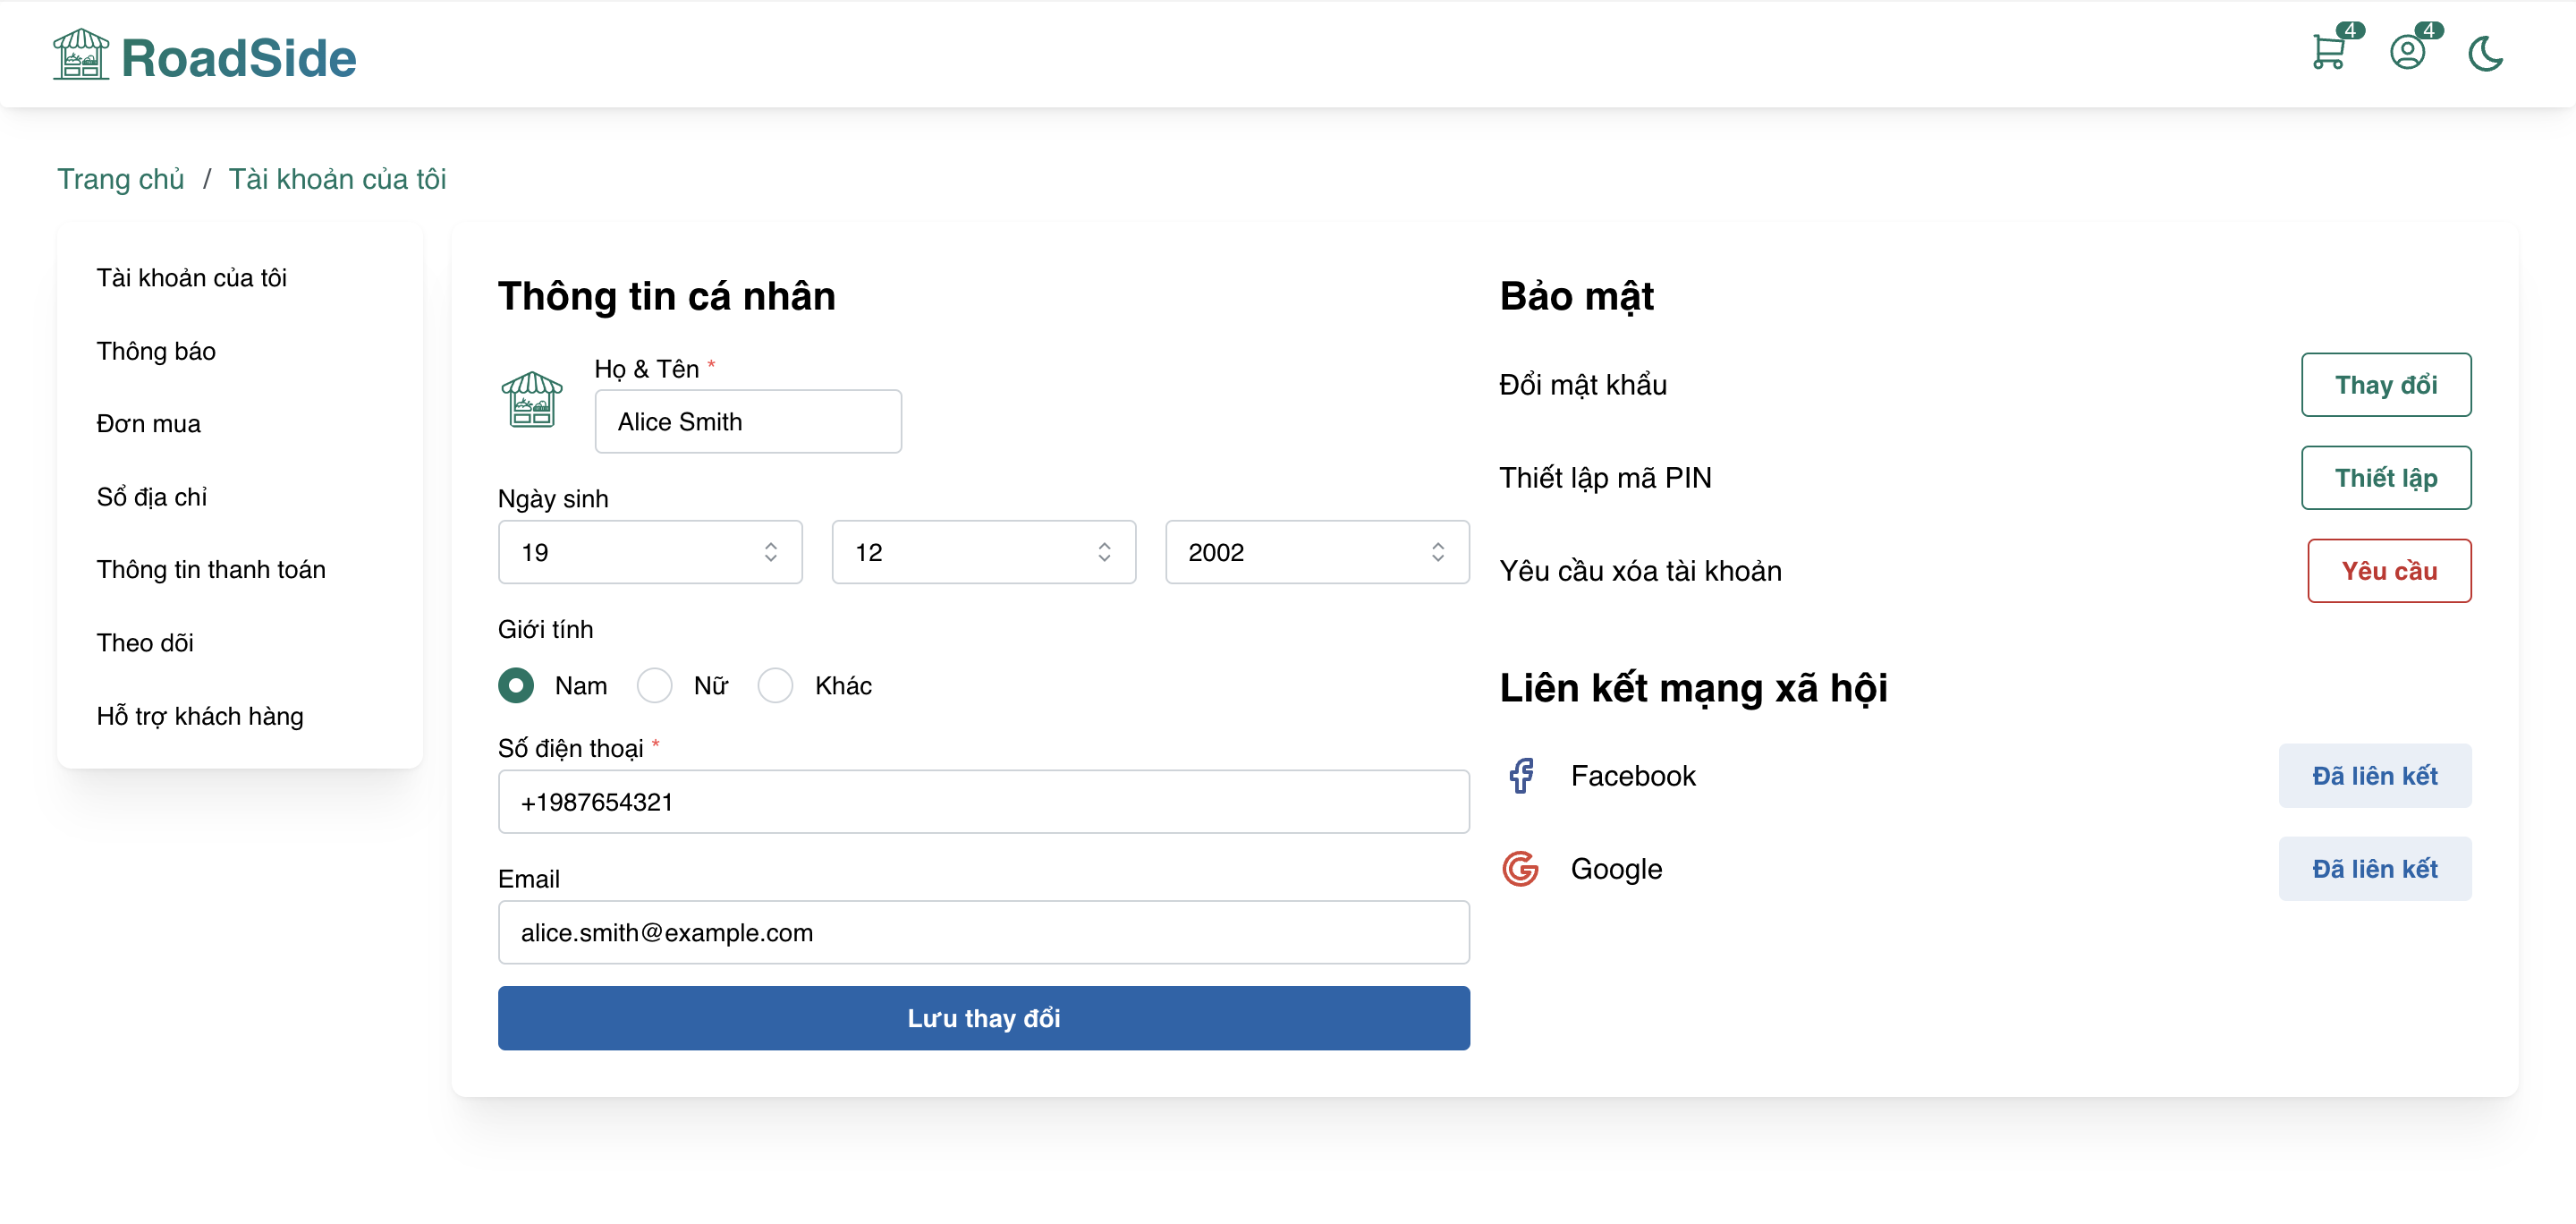
\includegraphics[scale=0.3] {Images/UI/info profile.png}
        \vspace{1em}
        \caption{Trang thông tin người dùng}
    \end{figure}
Trang thông tin người dùng cũng cung cấp khả năng thay đổi mật khẩu. Điều này cho phép người dùng cập nhật mật khẩu của mình một cách an toàn và bảo mật.

Người dùng cũng có thể thiết lập nhiều địa chỉ cho tài khoản của mình.  

\begin{figure}[H]
    \centering
    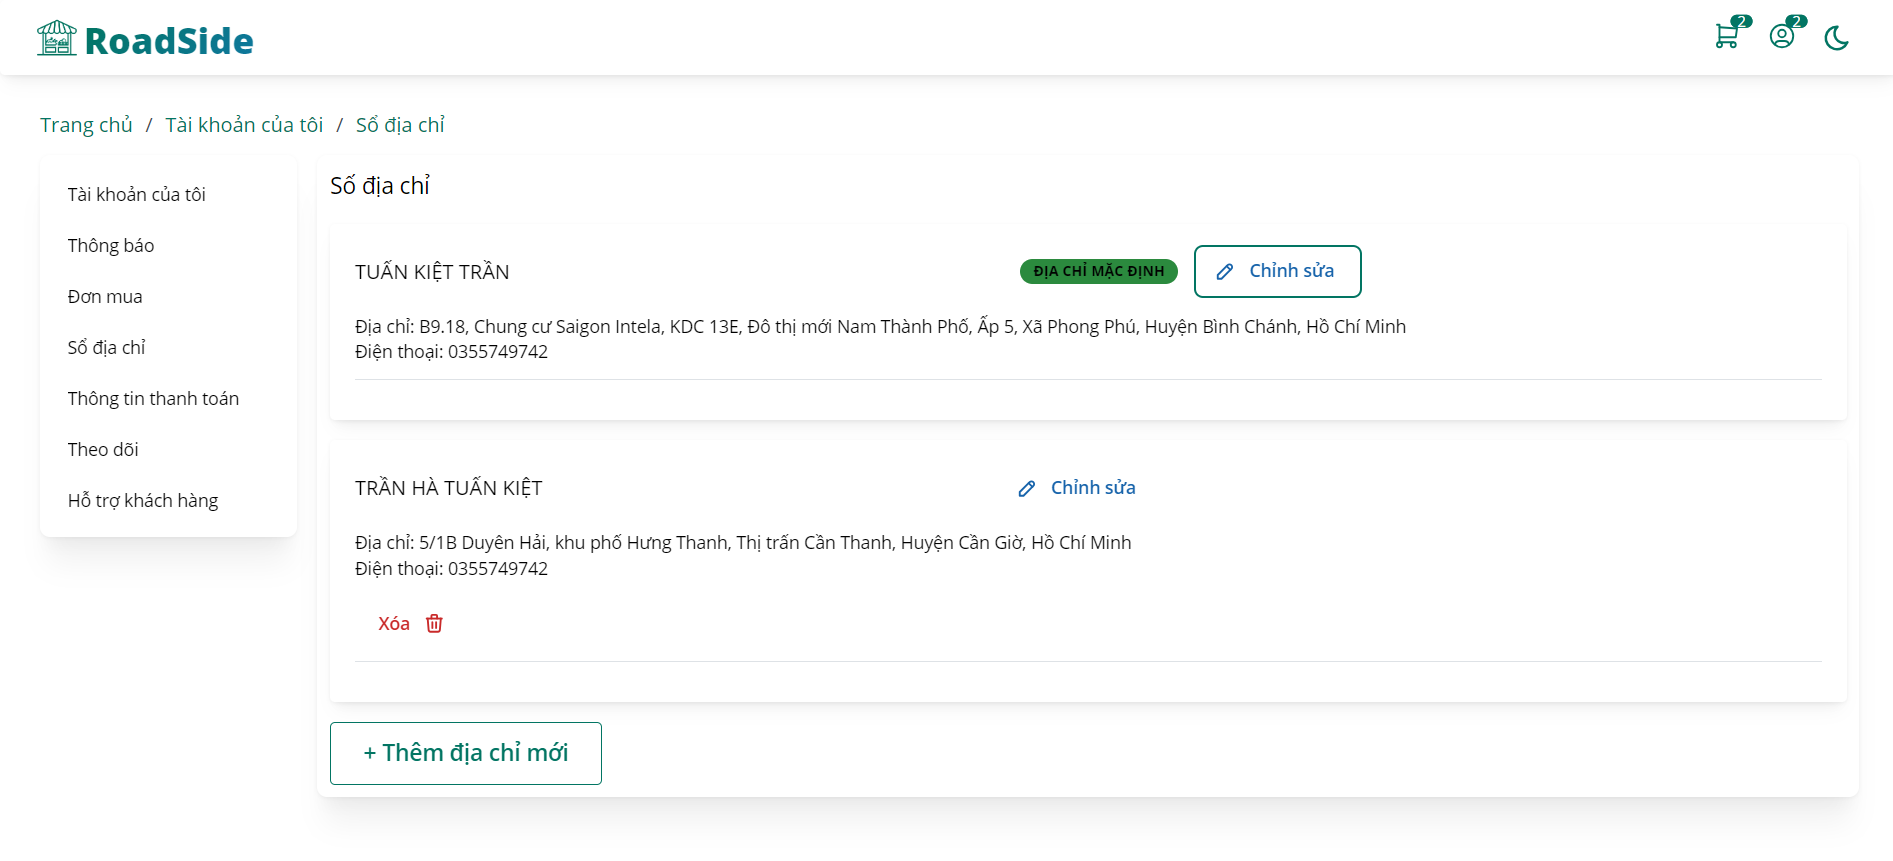
\includegraphics[scale=0.3] {Images/UI/address.png}
    \vspace{1em}
    \caption{Địa chỉ người dùng}
\end{figure}
\subsection{Quản lý đơn đặt hàng}
Ở trang profile cũng cung cấp thông tin đơn hàng của người dùng, bao gồm các thông tin về đơn hàng đang trong quá trình vận chuyển hoặc các đơn đã hoàn thành trước đây như số đơn hàng, ngày đặt hàng, sản phẩm đã mua và trạng thái đơn hàng. Điều này giúp người dùng theo dõi và quản lý các đơn hàng của họ một cách thuận tiện.
    \begin{figure}[H]
        \centering
        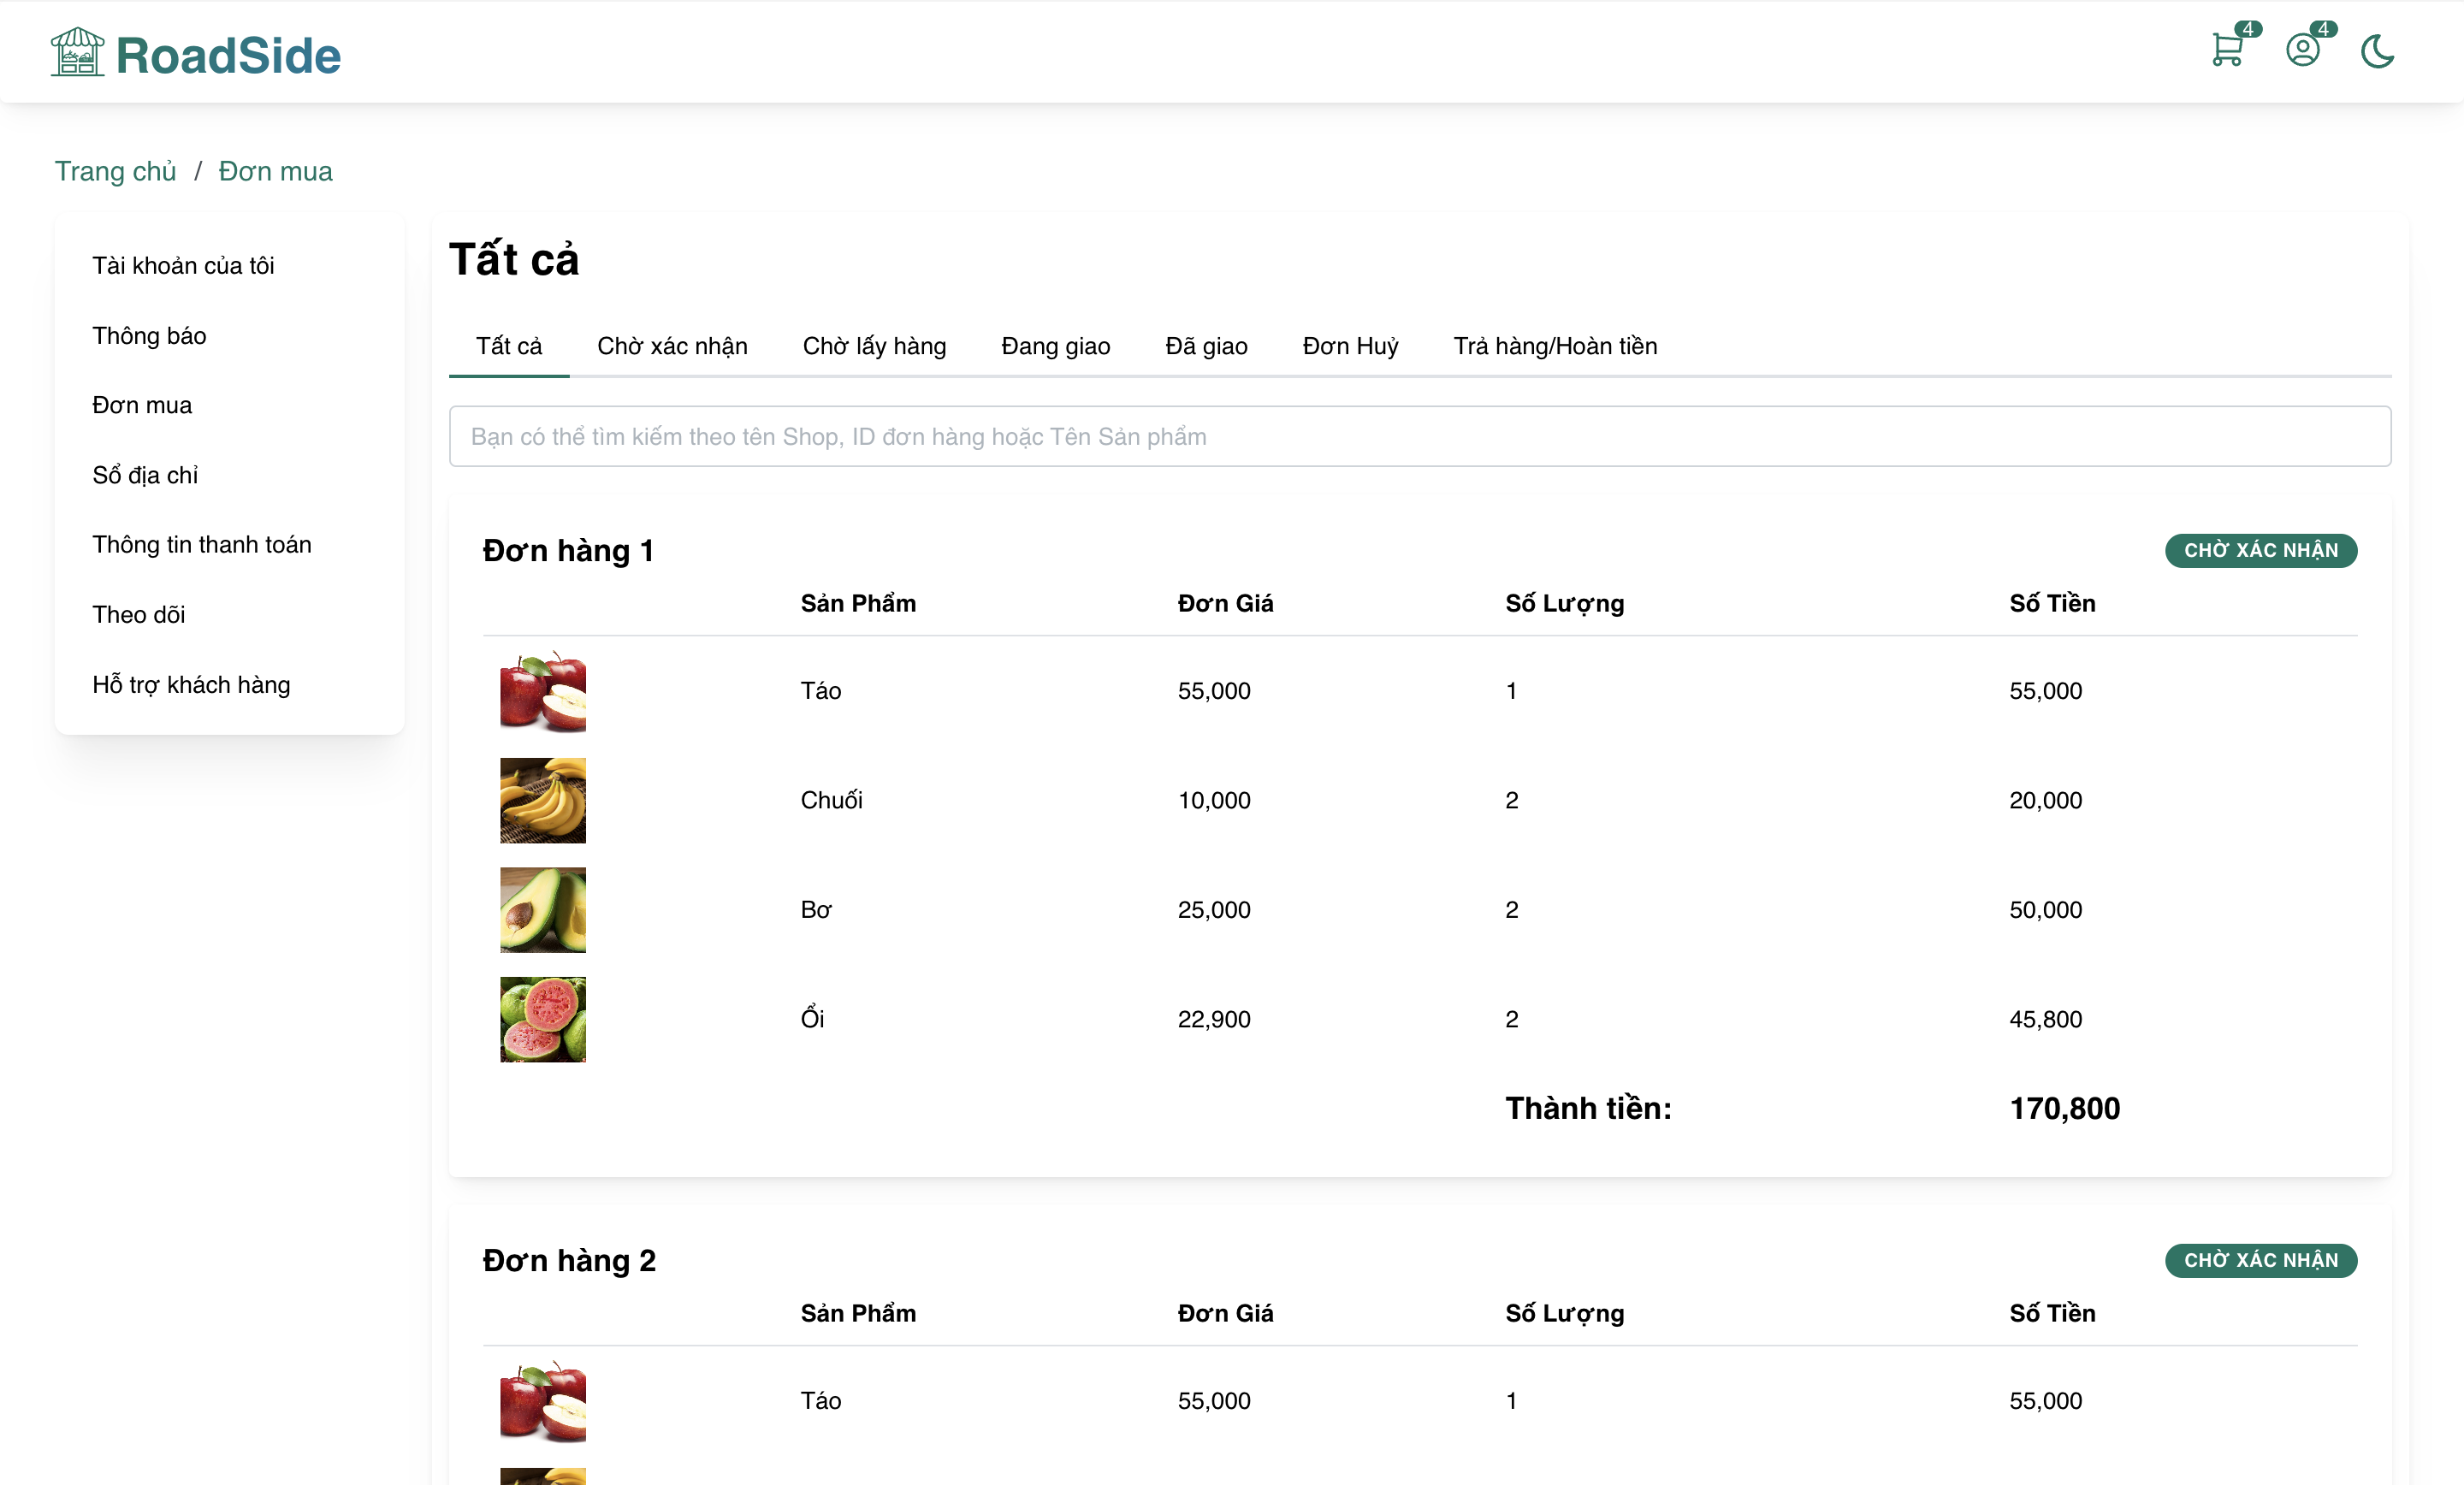
\includegraphics[width=\linewidth] {Images/UI/client order.png}
        \vspace{1em}
        \caption{Trang thông tin người dùng - Quản lý đơn hàng}
    \end{figure}
\subsection{Kênh cho chủ cửa hàng}
Mỗi tài khoản đều có thể tạo của hàng riêng cho mình, sẽ có một số trang riêng cho người dùng để quản lý cửa hàng và sản phẩm.
\begin{itemize}
    \item Quản lý sản phẩm:
    \begin{itemize}
        \item Tính năng quản lý sản phẩm cho phép chủ cửa hàng xem và quản lý các sản phẩm hiện có trong cửa hàng. Mỗi sản phẩm sẽ được hiển thị với các thông tin cơ bản như mã sản phẩm, tên, loại, giá, số lượng tồn kho và trạng thái hiện tại của sản phẩm. Ngoài ra, chủ cửa hàng cũng có thể xóa hay chỉnh sửa thông tin sản phẩm ở trang này.
        \begin{figure}[H]
            \centering
            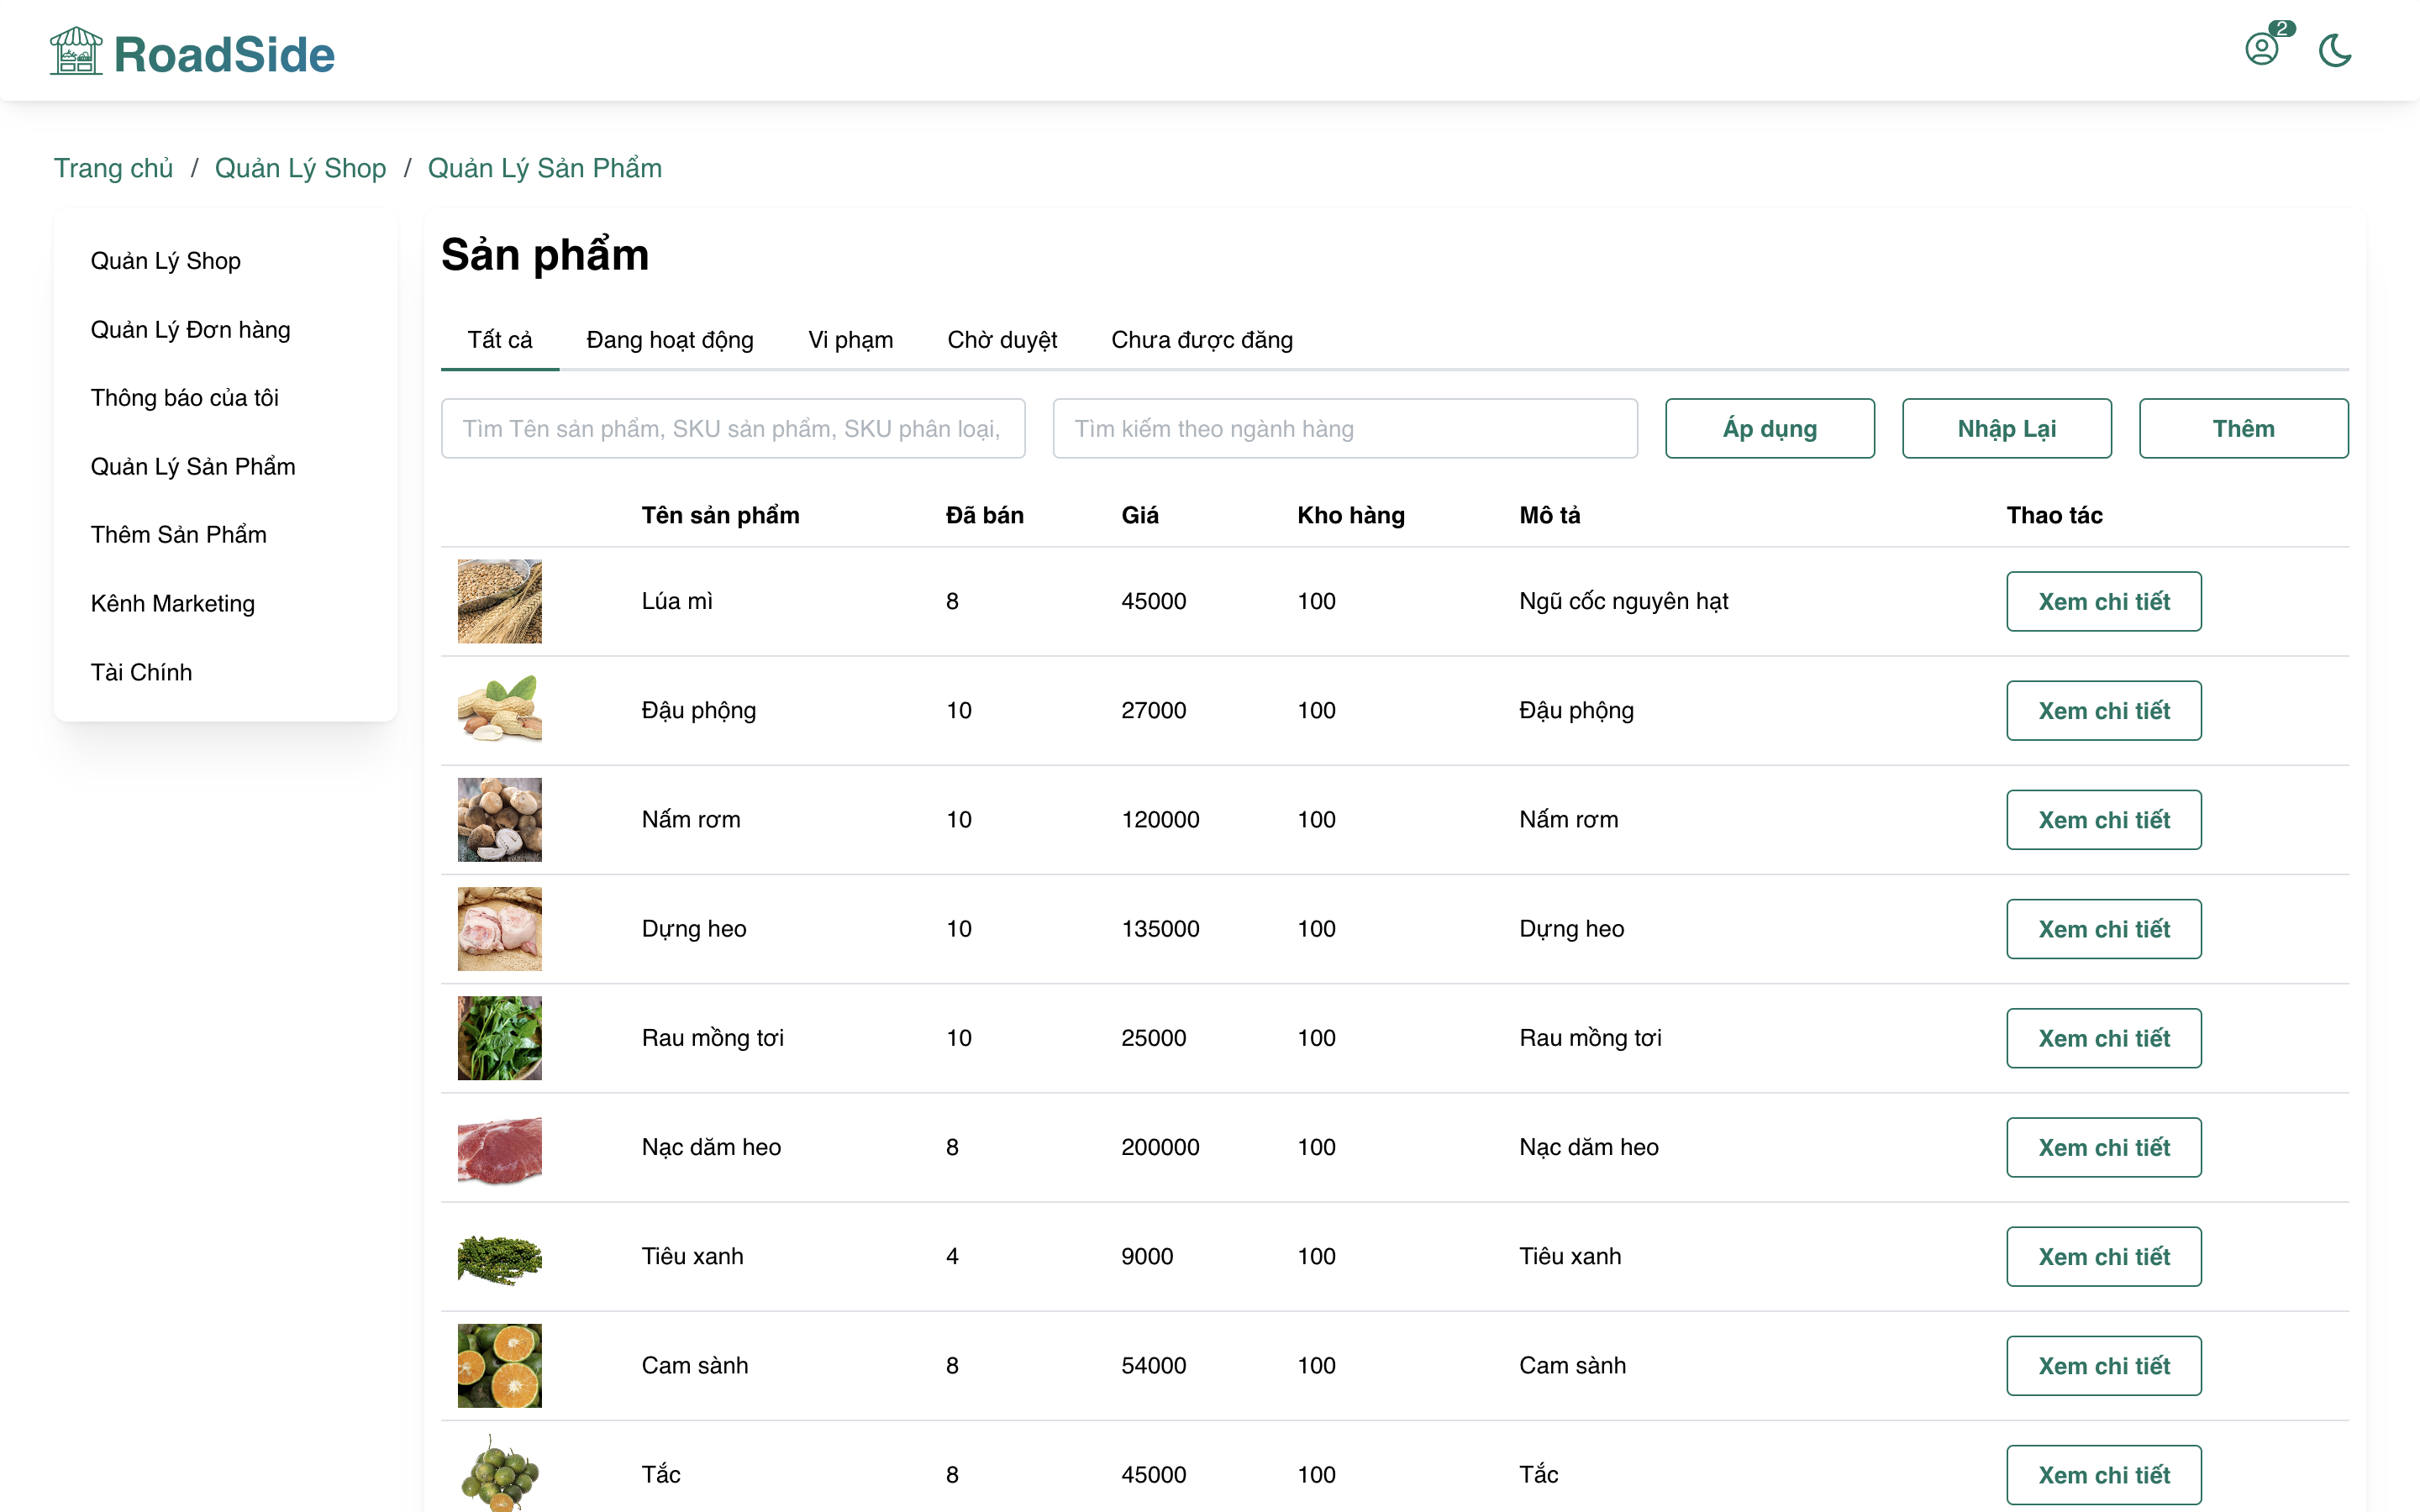
\includegraphics[width=0.95\linewidth] {Images/UI/shop_products.png}
            \vspace{1em}
            \caption{Quản lý sản phẩm}
        \end{figure}
        \item Chủ cửa hàng có thể lọc và tìm kiếm sản phẩm theo tên cũng như các đặc điểm khác.
        \item Thông tin của sản phẩm cũng có thể được chỉnh sửa ở đây.
    \end{itemize}
    \item Thêm sản phẩm mới: Chủ cửa hàng có thể thêm sản phẩm mới cho cửa hàng của mình thông qua tính năng này. Trong trang thêm sản phẩm, chủ cửa hàng sẽ phải điền một form với các trường thông tin chi tiết về sản phẩm như tên, hình ảnh, loại, mô tả,... 
        \begin{figure}[H]
            \begin{center}
            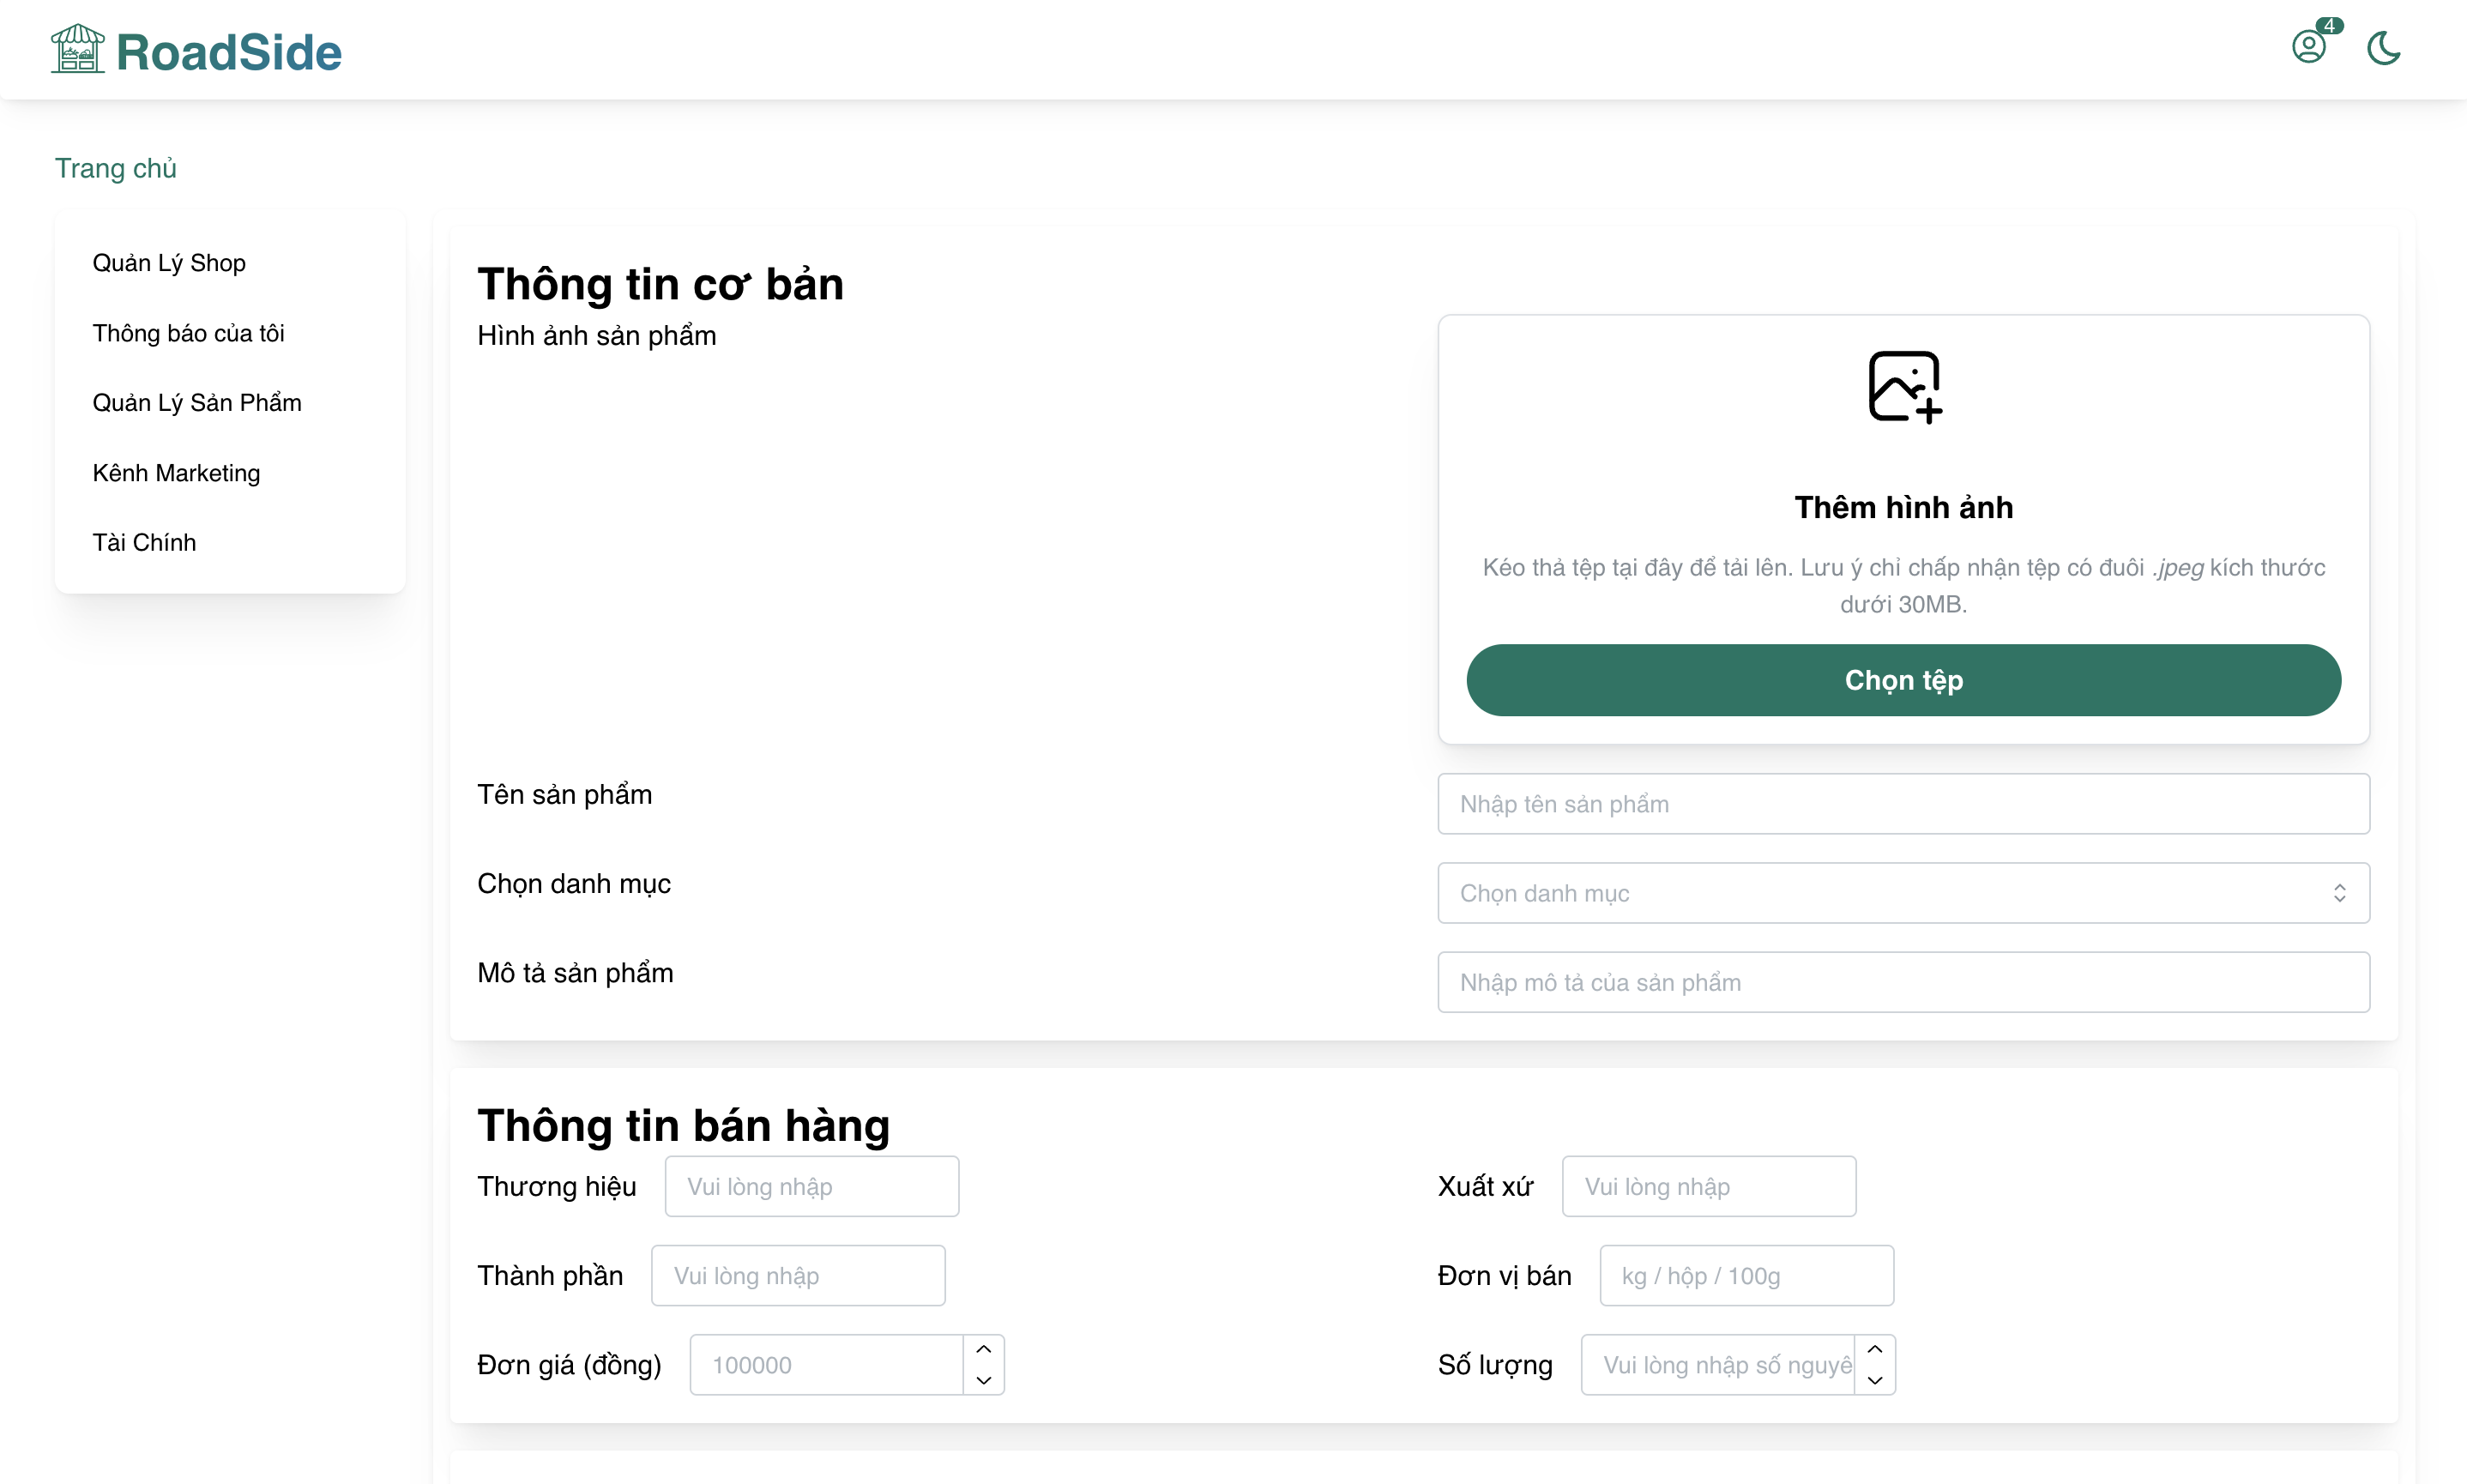
\includegraphics[width=\linewidth] {Images/UI/shop_addproduct.png}
            \end{center}
            \caption{Thêm sản phẩm mới}
        \end{figure}
\end{itemize}

\subsection{Chế độ sáng - tối}
Ngoài ra trang web còn hỗ trợ chuyển đổi chế độ sáng - tối cho giao diện.
\begin{figure}[H]
    \centering
    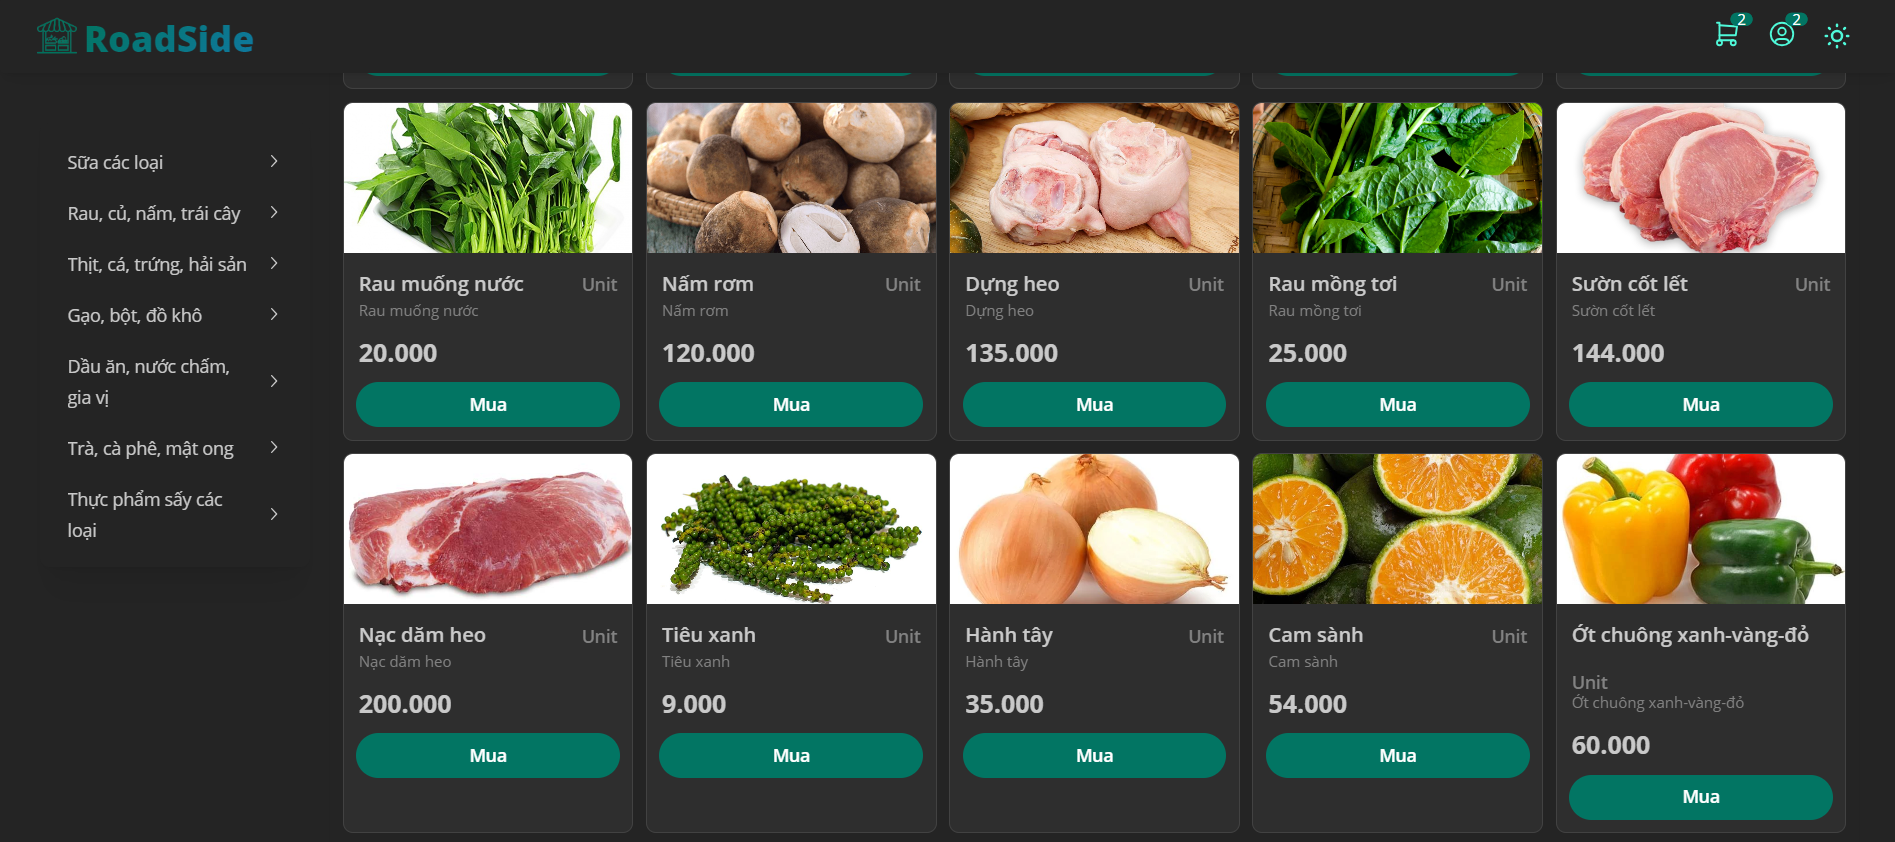
\includegraphics[width=0.95\linewidth] {Images/UI/darkmode1.png}
\end{figure}
\begin{figure}[H]
    \centering
    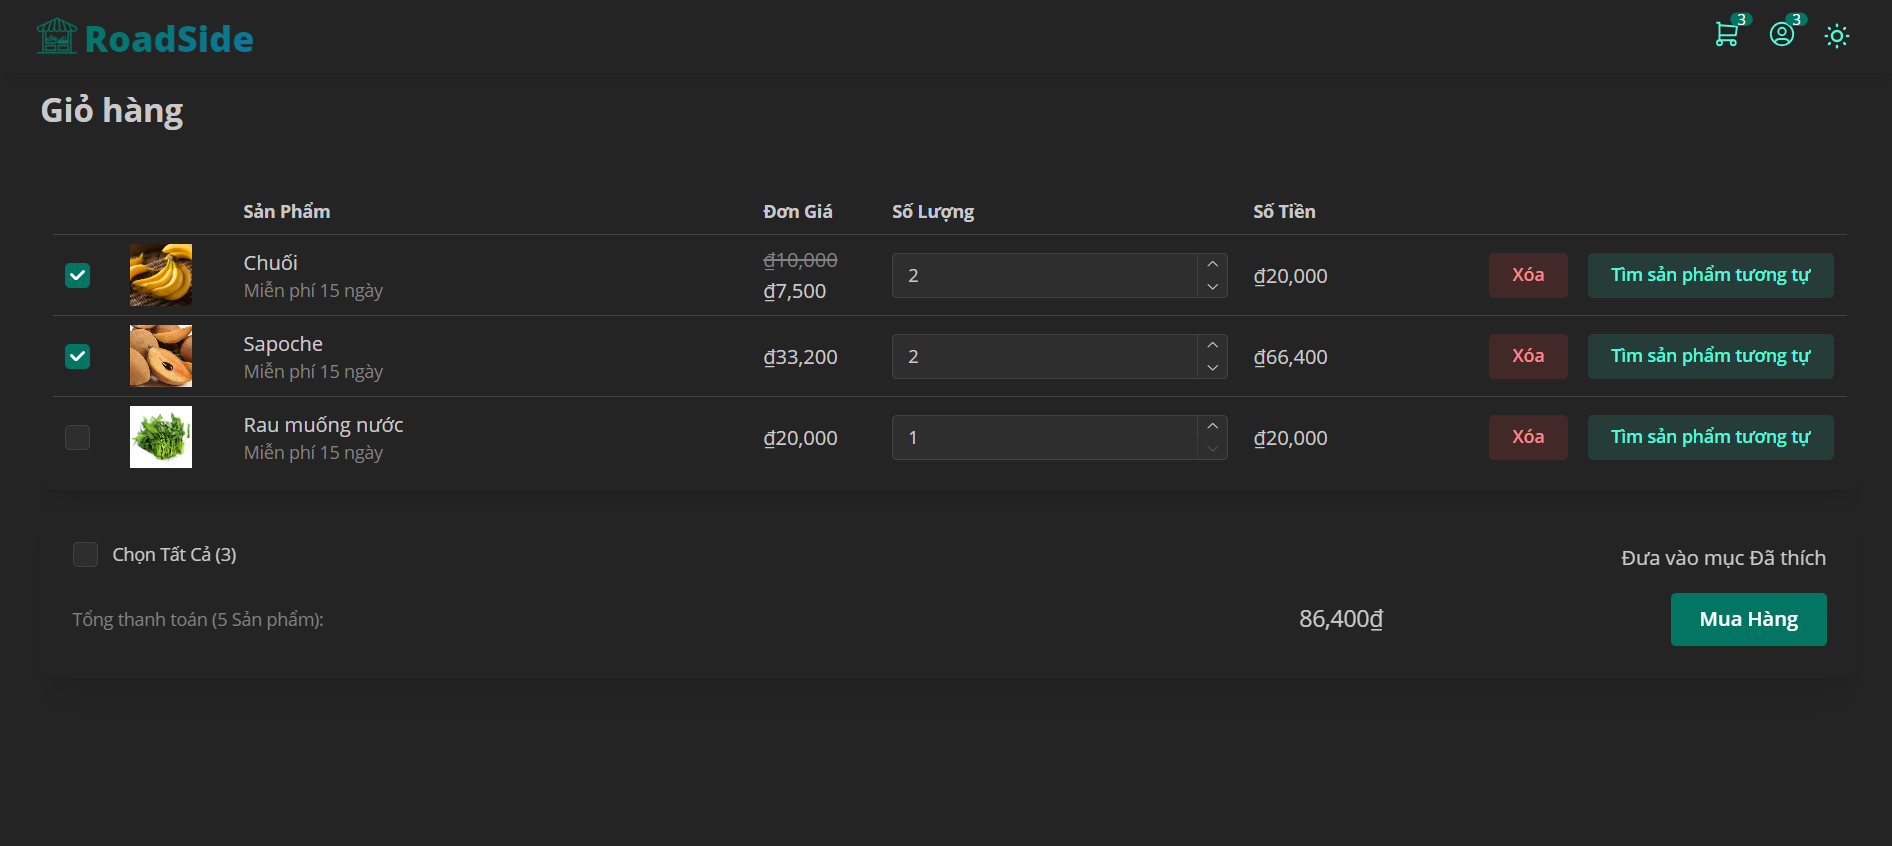
\includegraphics[width=0.95\linewidth] {Images/UI/darkmode2.png}
\end{figure}
\begin{figure}[H]
    \centering
    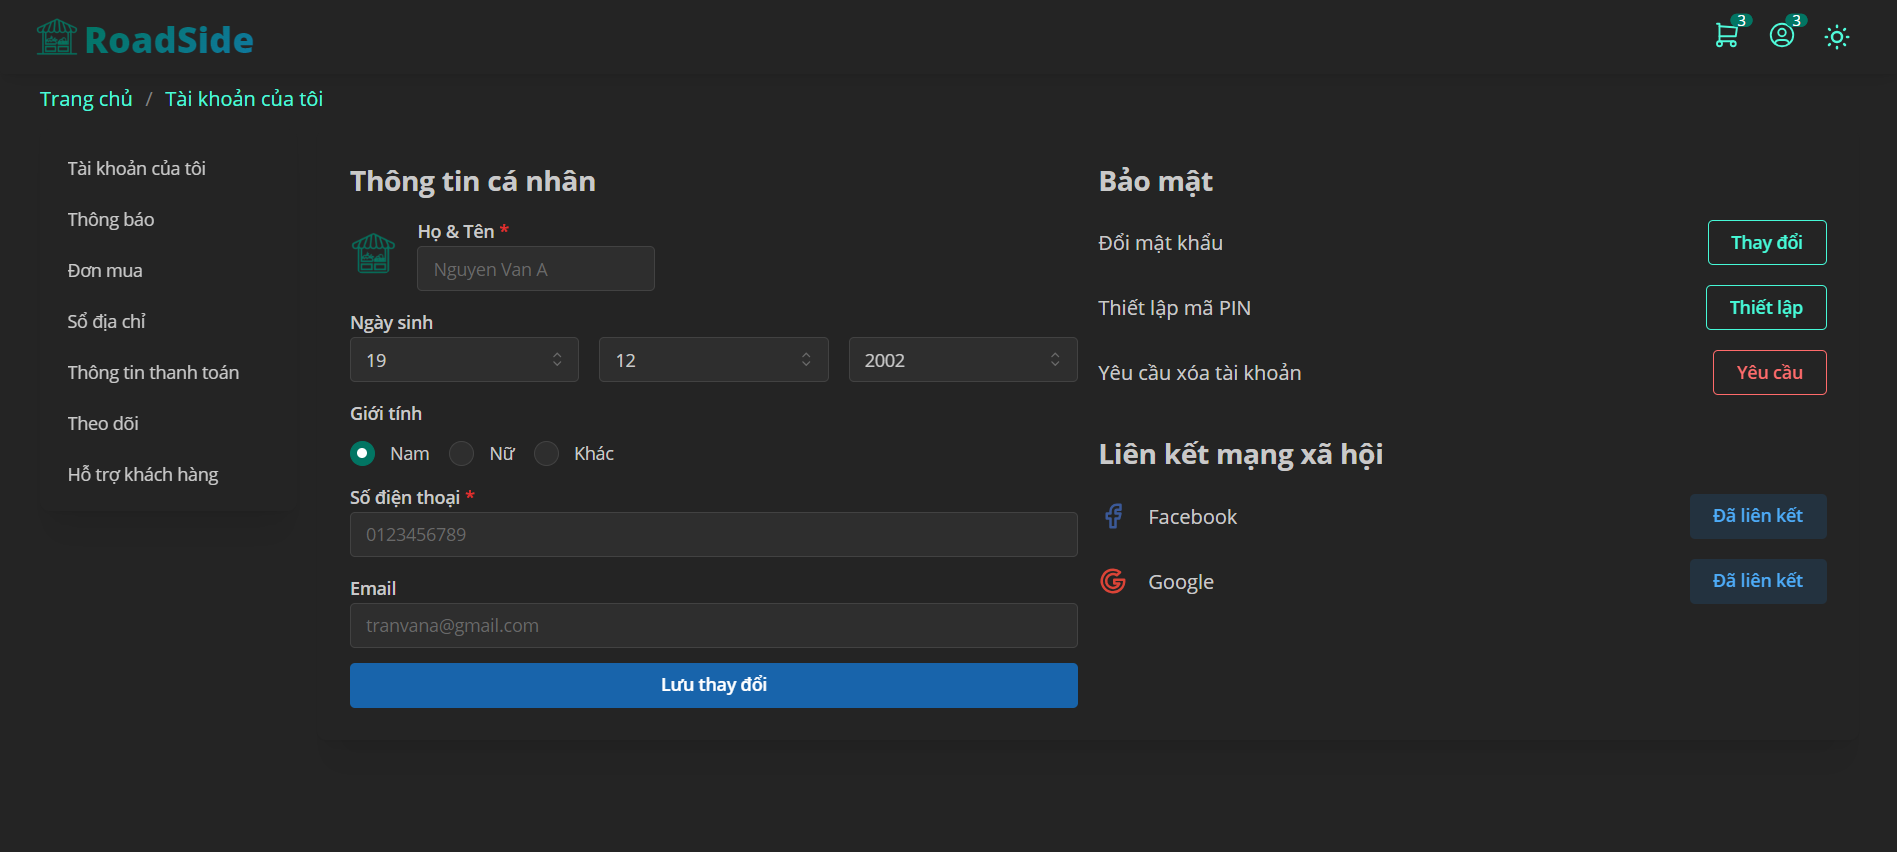
\includegraphics[width=0.95\linewidth] {Images/UI/darkmode3.png}
    \vspace{1em}
    \caption{Một số trang ở chế độ tối}
\end{figure}